% Options for packages loaded elsewhere
\PassOptionsToPackage{unicode}{hyperref}
\PassOptionsToPackage{hyphens}{url}
\PassOptionsToPackage{dvipsnames,svgnames,x11names}{xcolor}
%
\documentclass[
  letterpaper,
  DIV=11,
  numbers=noendperiod]{scrartcl}

\usepackage{amsmath,amssymb}
\usepackage{iftex}
\ifPDFTeX
  \usepackage[T1]{fontenc}
  \usepackage[utf8]{inputenc}
  \usepackage{textcomp} % provide euro and other symbols
\else % if luatex or xetex
  \usepackage{unicode-math}
  \defaultfontfeatures{Scale=MatchLowercase}
  \defaultfontfeatures[\rmfamily]{Ligatures=TeX,Scale=1}
\fi
\usepackage{lmodern}
\ifPDFTeX\else  
    % xetex/luatex font selection
\fi
% Use upquote if available, for straight quotes in verbatim environments
\IfFileExists{upquote.sty}{\usepackage{upquote}}{}
\IfFileExists{microtype.sty}{% use microtype if available
  \usepackage[]{microtype}
  \UseMicrotypeSet[protrusion]{basicmath} % disable protrusion for tt fonts
}{}
\makeatletter
\@ifundefined{KOMAClassName}{% if non-KOMA class
  \IfFileExists{parskip.sty}{%
    \usepackage{parskip}
  }{% else
    \setlength{\parindent}{0pt}
    \setlength{\parskip}{6pt plus 2pt minus 1pt}}
}{% if KOMA class
  \KOMAoptions{parskip=half}}
\makeatother
\usepackage{xcolor}
\setlength{\emergencystretch}{3em} % prevent overfull lines
\setcounter{secnumdepth}{5}
% Make \paragraph and \subparagraph free-standing
\ifx\paragraph\undefined\else
  \let\oldparagraph\paragraph
  \renewcommand{\paragraph}[1]{\oldparagraph{#1}\mbox{}}
\fi
\ifx\subparagraph\undefined\else
  \let\oldsubparagraph\subparagraph
  \renewcommand{\subparagraph}[1]{\oldsubparagraph{#1}\mbox{}}
\fi


\providecommand{\tightlist}{%
  \setlength{\itemsep}{0pt}\setlength{\parskip}{0pt}}\usepackage{longtable,booktabs,array}
\usepackage{calc} % for calculating minipage widths
% Correct order of tables after \paragraph or \subparagraph
\usepackage{etoolbox}
\makeatletter
\patchcmd\longtable{\par}{\if@noskipsec\mbox{}\fi\par}{}{}
\makeatother
% Allow footnotes in longtable head/foot
\IfFileExists{footnotehyper.sty}{\usepackage{footnotehyper}}{\usepackage{footnote}}
\makesavenoteenv{longtable}
\usepackage{graphicx}
\makeatletter
\def\maxwidth{\ifdim\Gin@nat@width>\linewidth\linewidth\else\Gin@nat@width\fi}
\def\maxheight{\ifdim\Gin@nat@height>\textheight\textheight\else\Gin@nat@height\fi}
\makeatother
% Scale images if necessary, so that they will not overflow the page
% margins by default, and it is still possible to overwrite the defaults
% using explicit options in \includegraphics[width, height, ...]{}
\setkeys{Gin}{width=\maxwidth,height=\maxheight,keepaspectratio}
% Set default figure placement to htbp
\makeatletter
\def\fps@figure{htbp}
\makeatother
% definitions for citeproc citations
\NewDocumentCommand\citeproctext{}{}
\NewDocumentCommand\citeproc{mm}{%
  \begingroup\def\citeproctext{#2}\cite{#1}\endgroup}
\makeatletter
 % allow citations to break across lines
 \let\@cite@ofmt\@firstofone
 % avoid brackets around text for \cite:
 \def\@biblabel#1{}
 \def\@cite#1#2{{#1\if@tempswa , #2\fi}}
\makeatother
\newlength{\cslhangindent}
\setlength{\cslhangindent}{1.5em}
\newlength{\csllabelwidth}
\setlength{\csllabelwidth}{3em}
\newenvironment{CSLReferences}[2] % #1 hanging-indent, #2 entry-spacing
 {\begin{list}{}{%
  \setlength{\itemindent}{0pt}
  \setlength{\leftmargin}{0pt}
  \setlength{\parsep}{0pt}
  % turn on hanging indent if param 1 is 1
  \ifodd #1
   \setlength{\leftmargin}{\cslhangindent}
   \setlength{\itemindent}{-1\cslhangindent}
  \fi
  % set entry spacing
  \setlength{\itemsep}{#2\baselineskip}}}
 {\end{list}}
\usepackage{calc}
\newcommand{\CSLBlock}[1]{\hfill\break\parbox[t]{\linewidth}{\strut\ignorespaces#1\strut}}
\newcommand{\CSLLeftMargin}[1]{\parbox[t]{\csllabelwidth}{\strut#1\strut}}
\newcommand{\CSLRightInline}[1]{\parbox[t]{\linewidth - \csllabelwidth}{\strut#1\strut}}
\newcommand{\CSLIndent}[1]{\hspace{\cslhangindent}#1}

\KOMAoption{captions}{tableheading}
\makeatletter
\@ifpackageloaded{caption}{}{\usepackage{caption}}
\AtBeginDocument{%
\ifdefined\contentsname
  \renewcommand*\contentsname{Table of contents}
\else
  \newcommand\contentsname{Table of contents}
\fi
\ifdefined\listfigurename
  \renewcommand*\listfigurename{List of Figures}
\else
  \newcommand\listfigurename{List of Figures}
\fi
\ifdefined\listtablename
  \renewcommand*\listtablename{List of Tables}
\else
  \newcommand\listtablename{List of Tables}
\fi
\ifdefined\figurename
  \renewcommand*\figurename{Figure}
\else
  \newcommand\figurename{Figure}
\fi
\ifdefined\tablename
  \renewcommand*\tablename{Table}
\else
  \newcommand\tablename{Table}
\fi
}
\@ifpackageloaded{float}{}{\usepackage{float}}
\floatstyle{ruled}
\@ifundefined{c@chapter}{\newfloat{codelisting}{h}{lop}}{\newfloat{codelisting}{h}{lop}[chapter]}
\floatname{codelisting}{Listing}
\newcommand*\listoflistings{\listof{codelisting}{List of Listings}}
\makeatother
\makeatletter
\makeatother
\makeatletter
\@ifpackageloaded{caption}{}{\usepackage{caption}}
\@ifpackageloaded{subcaption}{}{\usepackage{subcaption}}
\makeatother
\ifLuaTeX
  \usepackage{selnolig}  % disable illegal ligatures
\fi
\usepackage{bookmark}

\IfFileExists{xurl.sty}{\usepackage{xurl}}{} % add URL line breaks if available
\urlstyle{same} % disable monospaced font for URLs
\hypersetup{
  pdftitle={Conditional Probability Theory},
  pdfauthor={Michael Betancourt},
  colorlinks=true,
  linkcolor={blue},
  filecolor={Maroon},
  citecolor={Blue},
  urlcolor={Blue},
  pdfcreator={LaTeX via pandoc}}

\title{Conditional Probability Theory}
\author{Michael Betancourt}
\date{February 2023}

\begin{document}
\maketitle

\renewcommand*\contentsname{Table of contents}
{
\hypersetup{linkcolor=}
\setcounter{tocdepth}{3}
\tableofcontents
}
\newcommand{\I}[2]{\mathbb{I}_{#1} \! \left[ #2 \right]}

\newcommand{\E}[2]{\mathbb{E}_{#1} \! \left[ #2 \right]}

\newcommand{\rnd}[2]{\frac{ \mathrm{d} #1}{ \mathrm{d} #2 }}

Conditional probability theory provides a rigorous way to decompose
probability distributions over a space \(X\) into a collection of
probability distributions over subsets of \(X\). This decomposition
introduces two powerful new operations into probability theory. Firstly
it allows us to reduce complicated probabilistic calculations over all
of \(X\) into a sequence of potentially-simpler calculations over the
smaller subsets. At the same time it also encodes the information that
we lose when pushing probability distributions forward along
non-bijective transformations. This, in turn, facilitates the practical
construction of probability distributions by allowing us to build them
up from more manageable, lower-dimensional components.

That said conditional probability theory can be subtle, and to avoid any
confusion our introduction we will need to proceed carefully. We will
first learn how to decompose spaces into subsets before discussing how
probability distributions can be decomposed across those subsets.
Finally we will dedicate a good bit of time working out how to decompose
the probability density functions that are so critical to practical
applications.

\section{Decomposing Spaces With Partitions}\label{sec:partitions}

In
\href{https://betanalpha.github.io/assets/chapters_html/density_functions.html\#sigma-finite-measures}{Chapter
6, Section 1.2.1} we introduced the notion of a \emph{partition}
(Figure~\ref{fig-partition-valid}): a collection of subsets \[
\mathcal{P}
= \{ \mathsf{c}_{1}, \ldots, \mathsf{c}_{i}, \ldots \},
\] that are non-empty, \[
\mathsf{c}_{i} \ne \emptyset,
\] are mutually disjoint, \[
\mathsf{c}_{i} \cap \mathsf{c}_{i' \ne i} = \emptyset,
\] and cover the entire space, \[
\cup_{i} \mathsf{c}_{i} = X.
\] A collection of subsets that cover \(X\) but intersect with each
other do not form a valid partition
(Figure~\ref{fig-partition-overlapping}), nor does a collection of
disjoint subsets that don't cover all of \(X\)
(Figure~\ref{fig-partition-meager}).

\begin{figure}

\begin{minipage}{0.05\linewidth}
~\end{minipage}%
%
\begin{minipage}{0.45\linewidth}

\centering{

\captionsetup{labelsep=none}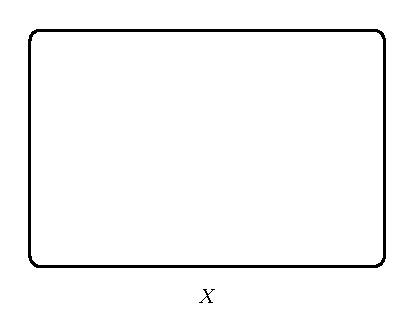
\includegraphics{figures/partitions/definition/space/space.pdf}

}

\subcaption{\label{fig-partition-space}}

\end{minipage}%
%
\begin{minipage}{0.45\linewidth}

\centering{

\captionsetup{labelsep=none}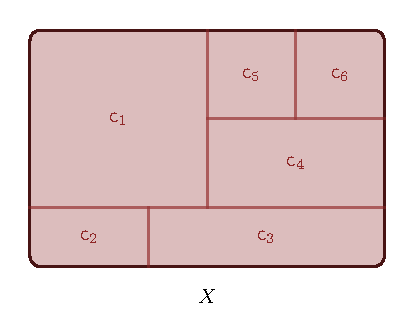
\includegraphics{figures/partitions/definition/valid/valid.pdf}

}

\subcaption{\label{fig-partition-valid}}

\end{minipage}%
%
\begin{minipage}{0.05\linewidth}
~\end{minipage}%
\newline
\begin{minipage}{0.05\linewidth}
~\end{minipage}%
%
\begin{minipage}{0.45\linewidth}

\centering{

\captionsetup{labelsep=none}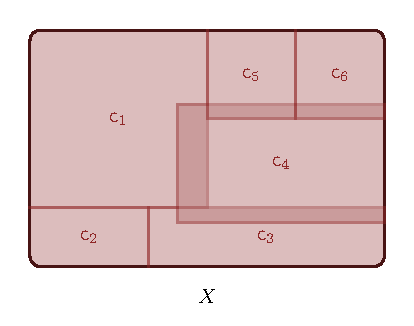
\includegraphics{figures/partitions/definition/overlapping/overlapping.pdf}

}

\subcaption{\label{fig-partition-overlapping}}

\end{minipage}%
%
\begin{minipage}{0.45\linewidth}

\centering{

\captionsetup{labelsep=none}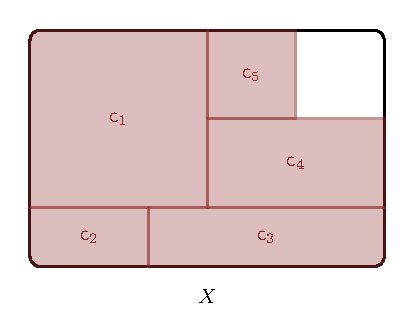
\includegraphics{figures/partitions/definition/meager/meager.pdf}

}

\subcaption{\label{fig-partition-meager}}

\end{minipage}%
%
\begin{minipage}{0.05\linewidth}
~\end{minipage}%

\caption{\label{fig-partition}A partition is a decomposition of (a) an
ambient space \(X\) into (b) a collection of disjoint subsets. (c)
Overlapping subsets that cover \(X\) do not form a proper partition, nor
do (d) disjoint subsets that do not fully cover \(X\). We can categorize
partitions by how many subsets they contain as well as the kinds of
subsets they contain. For example a measurable partition consists
entirely of disjoint subsets from the ambient \(\sigma\)-algebra,
\(\mathcal{X}\).}

\end{figure}%

The individual subsets that form a partition are known as the
\textbf{cells} of the partition. A partition can contain a finite number
of cells, a countably infinite number of cells, or even an uncountably
infinite number of cells. I will refer to partitions with a finite,
countably infinite, and uncountable infinite number of cells as finite,
countable, and uncountable partitions, respectively.

A finite partition can always be defined as an explicit list of cells,
but this isn't practical for countable or uncountable partitions which
would require infinitely long lists. In all of these cases, however, we
can \emph{implicitly} define a partition from the level sets of an
appropriate function.

Consider, for example, a finite partition \(\mathcal{P}\) defined as an
explicit list of \(I\) subsets, \[
\mathcal{P}
=
\{ \mathsf{c}_{1}, \ldots, \mathsf{c}_{i}, \ldots \mathsf{c}_{I} \}.
\] In order to distinguish between the individual cells I have assigned
them each a unique numerical label or \textbf{index} from the integers
\(\{1, \ldots, I \}\). Beyond a notational convenience, we can also use
this indexing to define the partition itself.

The indexing implicitly defines a bijective \textbf{index function} that
maps each cell to its corresponding integer index, \begin{alignat*}{6}
\chi_{\mathcal{P}}
:\; &\mathcal{P}& &\rightarrow& \; &\{1, \ldots, I \}&
\\
&\mathsf{c}_{i}& &\mapsto& &i&.
\end{alignat*} At the same time we can also define an \textbf{inclusion
function} that maps each point in the ambient space \(x \in X\) into the
partition cell that contains it, \begin{alignat*}{6}
\iota_{\mathcal{P}}
:\; &X& &\rightarrow& \; &\mathcal{P}&
\\
&x& &\mapsto&
&\{ \mathsf{c}_{i} \in \mathcal{P} \mid x \in \mathsf{c}_{i} \}&.
\end{alignat*} Composing these two functions together defines a third
function that maps points in the ambient space to partition cell indices
(Figure~\ref{fig-index-maps}), \begin{alignat*}{6}
\phi_{\mathcal{P}} = \chi_{\mathcal{P}} \circ \iota_{\mathcal{P}}
:\; &X& &\rightarrow& \; &\{1, \ldots, I \}&
\\
&x& &\mapsto&
&\{ i \in \{1, \ldots, I \} \mid
    x \in \mathsf{c}_{i} \in \mathcal{P} \}&.
\end{alignat*}

\begin{figure}

\centering{

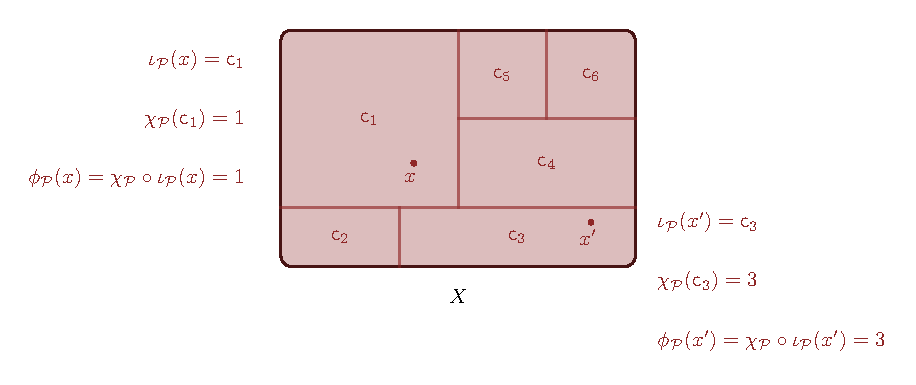
\includegraphics[width=0.9\textwidth,height=\textheight]{figures/partitions/indexing/maps/maps.pdf}

}

\caption{\label{fig-index-maps}Any finite partition of a space \(X\),
here \(\mathcal{P} =
\{ \mathsf{c}_{1}, \ldots, \mathsf{c}_{6} \}\), implicitly defines three
functions. The function \(\iota_{\mathcal{P}}\) maps each point \(X\) to
the partition cell that contains it while the function
\(\chi_{\mathcal{P}}\) maps each partition cell to its integer index.
The composition
\(\phi_{\mathcal{P}} = \chi_{\mathcal{P}} \circ \iota_{\mathcal{P}}\)
maps each point directly to the corresponding index.}

\end{figure}%

Because the partition cells are, by definition, disjoint and cover all
of \(X\) each point \(x \in X\) falls into one, and only one, partition
cell. In other words each point is associated with one and only one
partition cell index and \(\phi_{\mathcal{P}}\) will always be a
surjective function.

The level set of \(\phi_{\mathcal{P}}\) for a given index \(i\) is then
the subset of all input points that fall into the \(i\)th partition
cell, \[
\phi_{\mathcal{P}}^{-1}(i)
= \{ x \in X \mid \varpi_{\mathcal{P}}(x) = i \}
= \mathsf{c}_{i}.
\] Consequently we can completely reconstruct the cells of the partition
\(\mathcal{P}\) from these level sets
(Figure~\ref{fig-index-level-sets}), \[
\mathcal{P} = \{ \mathsf{c}_{1} = \varpi_{\mathcal{P}}^{-1}(1), \ldots,
                 \mathsf{c}_{i} = \varpi_{\mathcal{P}}^{-1}(i), \ldots,
                 \mathsf{c}_{I} = \varpi_{\mathcal{P}}^{-1}(I) \}!
\]

Because the cells in a partition are unordered the exact indexing we use
is arbitrary. Different permutations of the labels define different
index functions \(\chi_{\mathcal{P}}\) and hence different composite
functions \(\phi_{\mathcal{P}}\). The level sets of these functions,
however, are always the same, allowing us to work with whichever
indexing might be most convenient in any given application.

\begin{figure}

\begin{minipage}{0.50\linewidth}

\centering{

\captionsetup{labelsep=none}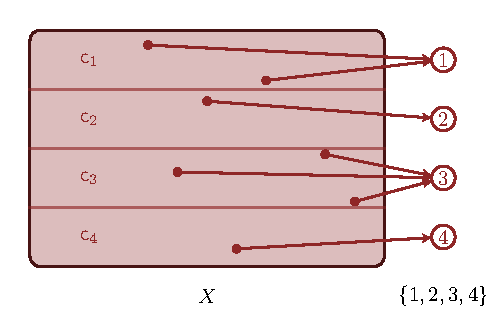
\includegraphics{figures/partitions/indexing/level_sets/forwards/forwards.pdf}

}

\subcaption{\label{fig-index-level-sets-forwards}}

\end{minipage}%
%
\begin{minipage}{0.50\linewidth}

\centering{

\captionsetup{labelsep=none}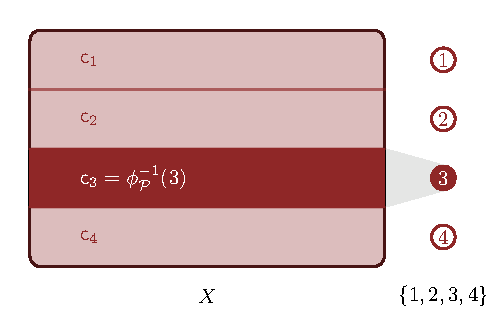
\includegraphics{figures/partitions/indexing/level_sets/backwards/backwards.pdf}

}

\subcaption{\label{fig-index-level-sets-backwards}}

\end{minipage}%

\caption{\label{fig-index-level-sets}The composite function (a)
\(\phi_{\mathcal{P}}\) maps points \(x \in X\) to the indices of the
partition cells that contain them. (b) The level sets
\(\phi_{\mathcal{P}}^{-1}(n)\) map each index to all of the points
contained in the corresponding partition cell. Collectively these level
sets completely reconstruct the initial partition,
\(\{ \phi_{\mathcal{P}}^{-1}(1), \phi_{\mathcal{P}}^{-1}(2),
   \phi_{\mathcal{P}}^{-1}(3), \phi_{\mathcal{P}}^{-1}(4) \}
= \{ \mathsf{c}_{1}, \mathsf{c}_{2}, \mathsf{c}_{3}, \mathsf{c}_{4} \}
= \mathcal{P}\).}

\end{figure}%

Let's take a breath and summarize what we've done so far. A finite
partition \(\mathcal{P}\) can be \emph{explicitly} defined as a list of
disjoint subsets or \emph{implicitly} defined by an appropriate
surjective function. The advantage of this implicit definition is that
it immediately generalizes to any type of partitions.

Every function \(f : X \rightarrow Y\) decomposes the input space \(X\)
into level sets \(f^{-1}(y)\) that are not only disjoint but also cover
all of \(X\), space, \[
X = \bigcup_{y \in Y} f^{-1}(y).
\] If \(f\) is surjective then every one if its level sets will also be
non-empty, \(f^{-1}(y) \ne \emptyset\) for all \(y \in Y\). Consequently
the level sets of \emph{every} surjective function implicitly defines a
partition where each cell is indexed by a unique output value.

If the output space \(Y\) contains a finite number of points then the
level sets of \(f\) define a finite partition
(Figure~\ref{fig-finite-partition}). On the other hand if \(Y\) contains
a countably infinite number of points then the level sets define a
countable partition even though we cannot exhaustively list every cell
in practice. Similarly if \(Y\) contains an uncountably infinite number
of points then the level sets define an uncountable partition
(Figure~\ref{fig-continuous-partition}).

\begin{figure}

\begin{minipage}{0.15\linewidth}
~\end{minipage}%
%
\begin{minipage}{0.70\linewidth}

\centering{

\captionsetup{labelsep=none}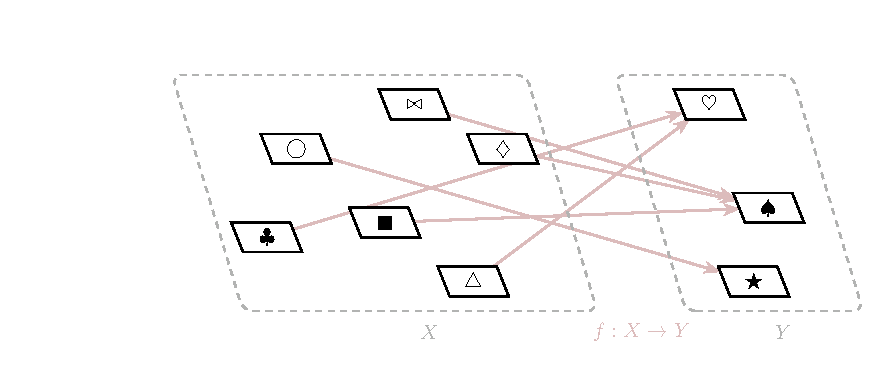
\includegraphics{figures/partitions/finite/function/function.pdf}

}

\subcaption{\label{fig-finite-partition-function}}

\end{minipage}%
%
\begin{minipage}{0.15\linewidth}
~\end{minipage}%
\newline
\begin{minipage}{0.15\linewidth}
~\end{minipage}%
%
\begin{minipage}{0.70\linewidth}

\centering{

\captionsetup{labelsep=none}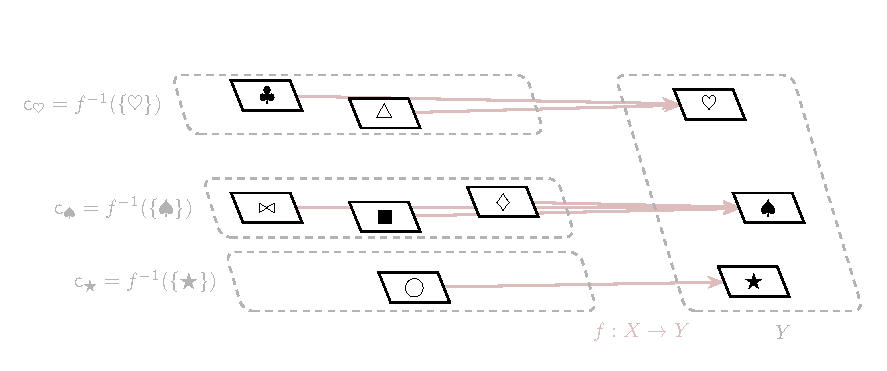
\includegraphics{figures/partitions/finite/table/table.pdf}

}

\subcaption{\label{fig-finite-partition-table}}

\end{minipage}%
%
\begin{minipage}{0.15\linewidth}
~\end{minipage}%

\caption{\label{fig-finite-partition}Every (a) surjective function
\(f : X \rightarrow Y\) with a finite output space defines (b) a finite
partition of the input space.}

\end{figure}%

\begin{figure}

\centering{

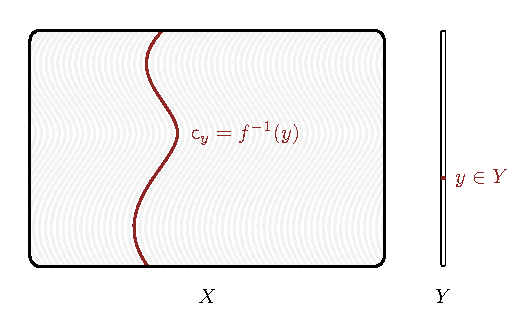
\includegraphics[width=0.6\textwidth,height=\textheight]{figures/partitions/continuous/continuous.pdf}

}

\caption{\label{fig-continuous-partition}Every surjective function
\(f : X \rightarrow Y\) with an uncountably infinite output space
defines an uncountable partition of the input space.}

\end{figure}%

To demonstrate uncountable partitions let's consider a few examples over
the space \(X = \mathbb{R}^{2}\). The surjective function
\begin{alignat*}{6}
f :\; &\mathbb{R}^{2}& &\rightarrow& \; &\mathbb{R}&
\\
&(x_{1}, x_{2})& &\mapsto& &x_{1}&
\end{alignat*} implicitly defines a partition that decomposes \(X\) into
an uncountable number of real lines, each of which can be visualized by
a vertical line (Figure~\ref{fig-partition-example-product}). Similarly
the surjective function \begin{alignat*}{6}
f :\; &\mathbb{R}^{2}& &\rightarrow& \; &\mathbb{R}^{+}&
\\
&(x_{1}, x_{2})& &\mapsto& &r = \sqrt{x_{1}^{2} + x_{2}^{2}}&
\end{alignat*} implicitly defines a partition that decomposes \(X\) into
an uncountable number of concentric arcs with a fixed radii
(Figure~\ref{fig-partition-example-radial}).

\begin{figure}

\begin{minipage}{0.50\linewidth}

\centering{

\captionsetup{labelsep=none}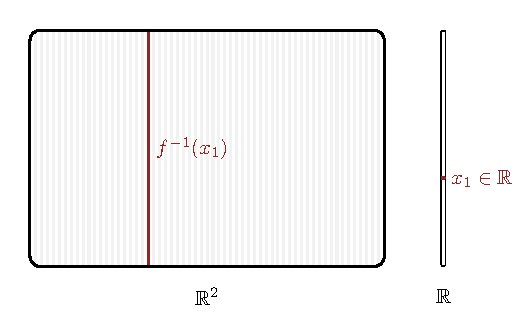
\includegraphics{figures/partitions/examples/product/product.pdf}

}

\subcaption{\label{fig-partition-example-product}}

\end{minipage}%
%
\begin{minipage}{0.50\linewidth}

\centering{

\captionsetup{labelsep=none}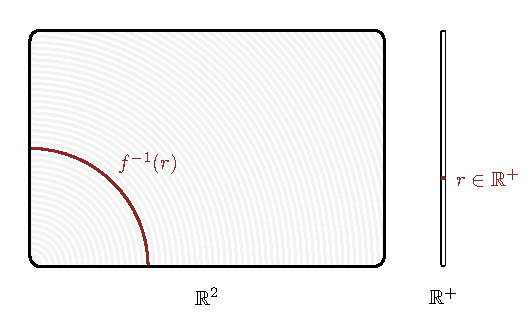
\includegraphics{figures/partitions/examples/radial/radial.pdf}

}

\subcaption{\label{fig-partition-example-radial}}

\end{minipage}%

\caption{\label{fig-partition-examples}The partitions defined by
surjective functions often admit convenient geometric interpretations.
(a) For example the function \(f : (x_{1}, x_{2}) \mapsto x_{1}\)
decomposes the ambient space \(\mathbb{R}^{2}\) into copies of
\(\mathbb{R}\), one for each output point \(x_{1} \in \mathbb{R}\). (b)
Likewise the function
\(f: (x_{1}, x_{2}) \mapsto \sqrt{x_{1}^{2} + x_{2}^{2} }\) decomposes
\(\mathbb{R}^{2}\) into concentric arcs.}

\end{figure}%

Partitions comprised of measurable subsets are particularly important in
probability theory. When the cells of a partition \(\mathcal{P}\) are
all \(\mathcal{X}\)-measurable the partition itself becomes a subset of
the defining \(\sigma\)-algebra, \(\mathcal{P} \subset \mathcal{X}\).
Unsurprisingly these partitions are referred to as
\textbf{\(\mathcal{X}\)-measurable partitions}, or simply
\textbf{measurable partitions} when the relevant \(\sigma\)-algebra is
unambiguous.

Even if a surjective function is measurable it may not define a
measurable partition. Only if the output space is equipped with a
\(\sigma\)-algebra \(\mathcal{Y}\) that includes all of the atomic
subsets, \[
\{ y \} \in \mathcal{Y}
\] for all \(y \in Y\), will the level sets of a measurable function
\(f : (X, \mathcal{X}) \rightarrow (Y, \mathcal{Y})\) always be
\(\mathcal{X}\)-measurable subsets of the input space, \[
f^{-1}( y ) = f^{*}( \{ y \} ) \in \mathcal{X}.
\] If \(\mathcal{Y}\) does contain all of the atomic subsets, however,
then every surjective and \((\mathcal{X}, \mathcal{Y})\)-measurable will
define measurable partition cells, and hence a measurable partition.

A \(\sigma\)-algebras that contains of all of the atomic subsets in the
ambient space is known as a \textbf{Hausdorff \(\sigma\)-algebra}.
Similarly a space paired with a Hausdorff \(\sigma\)-algebra is known as
a \textbf{Hausdorff measurable space}.

Fortunately all but the most pathological \(\sigma\)-algebras are
Hausdorff, and we can pretty safely assume that every \(\sigma\)-algebra
that we will encounter in practice will satisfy this property. Because
all of the functions that we will work with will be measurable we can
also safely assume that the partitions implicitly defined by any
surjective function we encounter in practice will be measurable.

\section{Conditioning on Countable And Explicit
Partitions}\label{sec:explicit-conditional}

Whether defined explicitly or implicitly, a partition decomposes a space
\(X\) into a collection of non-empty, non-overlapping subsets. This
spatial decomposition then provides the basis for decomposing
probability distributions over \(X\) into a collection of probability
distributions confined to those subsets. Before tackling the full
generality of this procedure we'll first build up intuition in the
simples case of countable partitions explicitly defined as lists of
subsets.

\subsection{The Law of Total
Probability}\label{the-law-of-total-probability}

As we saw in
\href{https://betanalpha.github.io/assets/chapters_html/probability_on_general_spaces.html}{Chapter
Four} Kolmogorov's axioms define a probability distribution as
consistent allocation of probability over measurable subsets.
Consequently in order to decompose a probability distribution we need to
be able to decompose measurables subset and the probabilities allocated
to them.

Any measurable set \(\mathsf{x} \in \mathcal{X}\) can be immediately
decomposed into its intersections with the cells of a given partition
\(\mathcal{P}\)
(Figure~\ref{fig-total-probability-subset-decomposition}), \[
\mathsf{x}
=
\bigcup_{\mathsf{c} \in \mathcal{P}}
\left( \mathsf{x} \cap \mathsf{c} \right).
\] Because the partition cells are mutually disjoint these intersections
will also be mutually disjoint: if \(\mathsf{c}_{1} \in \mathcal{P}\)
and \(\mathsf{c}_{2} \in \mathcal{P}\) are two distinct partition cells
then \begin{align*}
( \mathsf{x} \cap \mathsf{c}_{1} ) \cap ( \mathsf{x} \cap \mathsf{c}_{2} )
&=
( \mathsf{x} \cap \mathsf{c}_{1} ) \cap ( \mathsf{c}_{2} \cap \mathsf{x}  )
\\
&=
\mathsf{x} \cap ( \mathsf{c}_{1} \cap \mathsf{c}_{2} ) \cap \mathsf{x}
\\
&=
\mathsf{x} \cap \emptyset \cap \mathsf{x}
\\
&= \emptyset.
\end{align*}

If the partition \(\mathcal{P}\) is countable then any measurable subset
\(\mathsf{x} \in \mathcal{X}\) will decompose into a countable number of
components. Moreover because \(\sigma\)-algebras are closed under
countable unions then each of these components will also be measurable
whenever the partition is measurable. Consequently we can apply the
countable additivity of probability distributions to the decomposition
of any measurable subset induced by a measurable, countable partition
(Figure~\ref{fig-total-probability-probability-decomposition}).

In other words the probability allocated to
\(\mathsf{x} \in \mathcal{X}\) decomposes into a sum of the
probabilities allocated to the disjoint partition intersections,
\begin{align*}
\pi(\mathsf{x})
&=
\pi \left( \bigcup_{\mathsf{c} \in \mathcal{P}}
           \left( \mathsf{x} \cap \mathsf{c} \right) \right)
\\
&=
\sum_{\mathsf{c} \in \mathcal{P}} \pi( \mathsf{x} \cap \mathsf{c} ).
\end{align*} This decomposition of probability allocations is referred
to as \textbf{the law of total probability}.

\begin{figure}

\begin{minipage}{0.50\linewidth}

\centering{

\captionsetup{labelsep=none}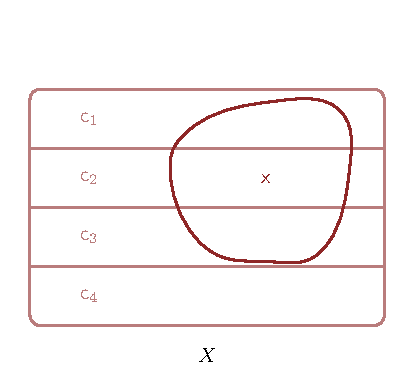
\includegraphics{figures/total_probability/subsets/subsets.pdf}

}

\subcaption{\label{fig-total-probability-subsets}}

\end{minipage}%
%
\begin{minipage}{0.50\linewidth}

\centering{

\captionsetup{labelsep=none}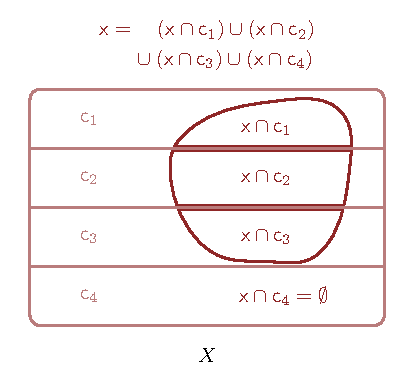
\includegraphics{figures/total_probability/subset_decomposition/subset_decomposition.pdf}

}

\subcaption{\label{fig-total-probability-subset-decomposition}}

\end{minipage}%
\newline
\begin{minipage}{0.25\linewidth}
~\end{minipage}%
%
\begin{minipage}{0.50\linewidth}

\centering{

\captionsetup{labelsep=none}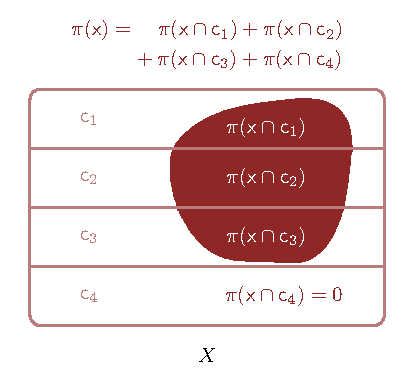
\includegraphics{figures/total_probability/probability_decomposition/probability_decomposition.pdf}

}

\subcaption{\label{fig-total-probability-probability-decomposition}}

\end{minipage}%
%
\begin{minipage}{0.25\linewidth}
~\end{minipage}%

\caption{\label{fig-total-probabilitity}Countable, measurable partitions
allow us to decompose probability allocations. (a) A measurable
partition decomposes \(X\) into four measurable subsets. (b) Every
measurable subset \(\mathsf{x} \subset \mathcal{X}\) decomposes into
disjoint intersections with the partition cells. (c) The probability
allocated to \(\mathsf{x}\) then decomposes into a sum of probabilities
allocated to each of these intersections.}

\end{figure}%

\subsection{Conditional Probabilities}\label{conditional-probabilities}

Now that we can decompose the probabilities allocated to individual
measurable subsets we can consider how to decompose entire probability
distributions. To make our first steps towards this decomposition more
manageable let's begin, however, with a simplifying restriction on the
partition.

Partitions whose cells are all allocated non-zero probabilities allow us
to multiply and divide by the cell probabilities without fear of
dividing by zero. I will refer to a partition where every cell is not
only measurable but also allocated a non-zero probability by the
probability distribution \(\pi\), \[
\pi(\mathsf{c}) > 0
\] for all \(\mathsf{c} \in \mathcal{P}\), as a
\textbf{\(\pi\)-non-null} partition.

Taking advantage of this flexibility we can rearrange each term in the
law of total probability to give \begin{align*}
\pi( \mathsf{x} )
&=
\sum_{\mathsf{c} \in \mathcal{P}} \pi( \mathsf{x} \cap \mathsf{c} )
\\
&=
\sum_{\mathsf{c} \in \mathcal{P}} \pi( \mathsf{x} \cap \mathsf{c} )
\cdot \frac{ \pi( \mathsf{c} ) }{ \pi( \mathsf{c} ) }
\\
&=
\sum_{\mathsf{c} \in \mathcal{P}}
\frac{ \pi(\mathsf{x} \cap \mathsf{c}) }{ \pi ( \mathsf{c} ) }
\cdot \pi( \mathsf{c} )
\\
&\equiv
\sum_{\mathsf{c} \in \mathcal{P}}
\pi^{\mathcal{P}}( \mathsf{x} \mid \mathsf{c} )
\cdot \pi( \mathsf{c} ).
\end{align*} Here each \textbf{conditional probability} \[
\pi^{\mathcal{P}}( \mathsf{x} \mid \mathsf{c} ) =
\frac{ \pi(\mathsf{x} \cap \mathsf{c}) }{ \pi (\mathsf{c}) }
\] quantifies the \emph{proportion} of the probability allocated to the
intersection of \(\mathsf{x}\) and the conditioning partition cell,
\(\pi(\mathsf{x} \cap \mathsf{c})\), relative to the total probability
allocated to the conditioning partition cell, \(\pi( \mathsf{c} )\)
(Figure Figure~\ref{fig-conditional-prob}).

\begin{figure}

\centering{

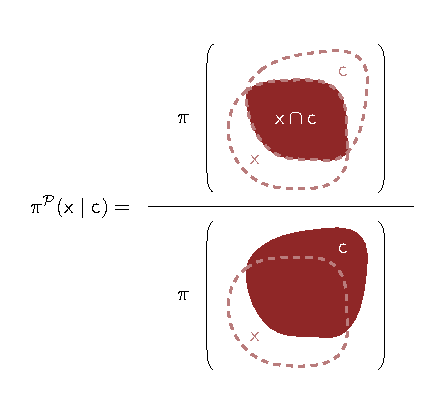
\includegraphics[width=0.6\textwidth,height=\textheight]{figures/conditional_probability/conditional_probability.pdf}

}

\caption{\label{fig-conditional-prob}The conditional probability of a
measurable subset \(\mathsf{x}\) given a measurable partition cell
\(\mathsf{c}\) quantifies the proportion of probability allocated to the
intersection \(\mathsf{x} \cap \mathsf{c}\) relative to the total
probability allocated to the partition cell \(\mathsf{c}\).}

\end{figure}%

By definition a measurable subset \(\mathsf{x} \in \mathcal{X}\) that
doesn't overlap with the conditioning partition cell \(\mathsf{c}\) is
allocated zero conditional probability, \begin{align*}
\pi^{\mathcal{P}}( \mathsf{x} \mid \mathsf{c} )
&=
\frac{ \pi(\mathsf{x} \cap \mathsf{c}) }{ \pi (\mathsf{c}) }
\\
&=
\frac{ \pi(\emptyset) }{ \pi (\mathsf{c}) }
\\
&=
\frac{ 0 }{ \pi (\mathsf{c}) }
\\
&=
0.
\end{align*} At the same time any measurable subset that completely
overlaps with the conditioning partition cell,
\(\mathsf{x} \cap \mathsf{c} = \mathsf{c}\), is allocated full
conditional probability, \begin{align*}
\pi^{\mathcal{P}}( \mathsf{x} \mid \mathsf{c} )
&=
\frac{ \pi(\mathsf{x} \cap \mathsf{c}) }{ \pi (\mathsf{c}) }
\\
&=
\frac{ \pi(\mathsf{c}) }{ \pi (\mathsf{c}) }
\\
&=
1.
\end{align*}

Conditional probabilities look suspiciously like probability allocations
that have been restricted to the domain of the conditioning partition
cell. With a little more work we can show that this suspicion is in fact
correct.

\subsection{Conditional Probability Distributions Over The Ambient
Space}\label{conditional-probability-distributions-over-the-ambient-space}

Given a measurable subset \(\mathsf{x} \in \mathcal{X}\) and a
measurable, \(\pi\)-non-null partition cell
\(\mathsf{c} \in \mathcal{P}\) we can construct a single conditional
probability \(\pi^{\mathcal{P}}( \mathsf{x} \mid \mathsf{c})\). The
collection of \emph{all} conditional probabilities relative to a
particular partition cell \(\mathsf{c}\) defines a function from
measurable subsets to conditional probabilities, \begin{alignat*}{6}
\pi^{\mathcal{P}}_{\mathsf{c}}
:\; &\mathcal{X}& &\rightarrow& \; &[0, 1]&
\\
&\mathsf{x} & &\mapsto&
&\frac{ \pi(\mathsf{x} \cap \mathsf{c}) }{ \pi (\mathsf{c}) }&.
\end{alignat*}

The immediate question is whether or not this function defines a
probability distribution. To answer that question we'll have to consider
the Kolmogorov axioms.

We begin with the first Kolmogorov axiom which requires a function that
maps measurable subsets into probabilities. This matches the inputs and
output spaces of \(\pi^{\mathcal{P}}_{\mathsf{c}}\).

In order to satisfy the second Kolmogorov axiom the probability
allocated to the entire ambient set must be one. Indeed \begin{align*}
\pi^{\mathcal{P}}_{\mathsf{c}}( X )
&=
\frac{ \pi(X \cap \mathsf{c}) }{ \pi(\mathsf{c}) }
\\
&=
\frac{ \pi(\mathsf{c}) }{ \pi(\mathsf{c}) }
\\
&=
1.
\end{align*}

Finally we need \(\pi^{\mathcal{P}}_{\mathsf{c}}\) to satisfy countable
additivity. For any countable collection of measurable but disjoint
subset sets \[
\{ \mathsf{x}_{1}, \ldots, \mathsf{x}_{j}, \ldots \}
\] we have \begin{align*}
\pi^{\mathcal{P}}_{\mathsf{c}}( \cup_{j} \mathsf{x}_{j} )
&=
\frac{ \pi( \, (\cup_{j} \mathsf{x}_{j}) \, \cap \mathsf{c}) }
{ \pi(\mathsf{c}) }
\\
&=
\frac{ \pi( \cup_{j} (\mathsf{x}_{j} \cap \mathsf{c}) ) }
{ \pi(\mathsf{c}) }
\\
&=
\frac{ \sum_{j} \pi( \mathsf{x}_{j} \cap \mathsf{c} ) }
{ \pi(\mathsf{c}) }
\\
&=
\sum_{j} \frac{ \pi( \mathsf{x}_{j} \cap \mathsf{c} ) }
{ \pi(\mathsf{c}) }
\\
&=
\sum_{j} \pi^{\mathcal{P}}_{\mathsf{c}}( \mathsf{x}_{j} ),
\end{align*} as needed.

With all three Kolmogorov axioms verified we can now formally state that
for any partition cell \(\mathsf{c}\) the function defined by \[
\pi^{\mathcal{P}}_{\mathsf{c}}( \mathsf{x} )
=
\frac{ \pi( \mathsf{x} \cap \mathsf{c}) }{ \pi (\mathsf{c}) }
\] defines a probability distribution over the ambient space \(X\).
Formally we say that \(\pi^{\mathcal{P}}_{\mathsf{c}}\) is a
\textbf{conditional probability distribution}.

\subsection{Conditional Probability Distributions Over Partition
Cells}\label{conditional-probability-distributions-over-partition-cells}

An important feature of conditional probability distributions is that
they much more singular than we might would expect from a probability
distribution over \(X\). Recall that any measurable subset that doesn't
intersect with the conditioning partition cell is always allocated zero
probability, \begin{align*}
\pi^{\mathcal{P}}_{\mathsf{c}}( \mathsf{x} )
&=
\pi^{\mathcal{P}}( \mathsf{x} \mid \mathsf{c} )
\\
&=
\frac{ \pi(\mathsf{x} \cap \mathsf{c}) }{ \pi(\mathsf{c}) }
\\
&=
\frac{ \pi(\emptyset) }{ \pi(\mathsf{c}) }
\\
&=
0.
\end{align*} Instead \emph{all} of the conditional probability
concentrates within the conditioning partition cell itself,
\begin{align*}
\pi^{\mathcal{P}}_{\mathsf{c}}( \mathsf{c} )
&=
\pi^{\mathcal{P}}( \mathsf{c} \mid \mathsf{c} )
\\
&=
\frac{ \pi(\mathsf{c} \cap \mathsf{c}) }{ \pi(\mathsf{c}) }
\\
&=
\frac{ \pi(\mathsf{c}) }{ \pi(\mathsf{c}) }
\\
&=
1!
\end{align*}

Intuitively this suggests that we can interpret a conditional
probability distribution as a \emph{restriction} of the initial
probability distribution to a particular partition cell. To formalize
this intuition, however, we have to define what it means to restrict not
only the elements of \((X, \mathcal{X})\) to a partition cell but also
the measurable subsets.

Taking the intersection of any subset \(\mathsf{x} \subset X\) with a
partition cell \(\mathsf{c} \subset X\) gives a subset whose elements
are entirely contained within the partition cell, \[
\mathsf{x} \cap \mathsf{c} \subset \mathsf{c}.
\] Moreover intersecting an entire collection of subsets \[
\{ \mathsf{x}_{1}, \ldots, \mathsf{x}_{j}, \ldots \} \subset 2^{X}
\] with \(\mathsf{c}\) gives a collection of subsets that are all
contained witin the partition cell, \[
\{ \mathsf{x}_{1} \cap \mathsf{c}, \ldots,
   \mathsf{x}_{j} \cap \mathsf{c}, \ldots \} \subset 2^{\mathsf{c}}.
\]

Importantly if the partition cell itself is an element of that initial
collection of subsets then this restriction respects the subset
operations. Formally if \(\mathcal{X} \subset 2^{X}\) is a collection of
subsets of \(X\) that contains \(\mathsf{c}\) and is closed under
complements, countable unions, and countable operations then the
collection of intersections \[
\mathcal{X}_{\mathsf{c}}
=
\{ \mathsf{x} \cap \mathsf{c} \text{ for all }
   \mathsf{x} \in \mathcal{X} \} \subset 2^{\mathsf{c}}
\] will also be a collection of subsets of \(\mathsf{c}\) that is closed
under complements, countable unions, and countable operations. In other
words if \(\mathcal{X}\) is a \(\sigma\)-algebra over \(X\) that
contains \(\mathsf{c}\) then \(\mathcal{X}_{\mathsf{c}}\) will be a
\(\sigma\)-algebra over \(\mathsf{c}\). This restricted
\(\sigma\)-algebra is known as a \textbf{subspace \(\sigma\)-algebra}.

By construction every measurable subset in a restricted
\(\sigma\)-algebra \(\mathcal{X}_{\mathsf{c}}\) is also a measurable
subset in the ambient \(\sigma\)-algebra \(\mathcal{X}\). Consequently
the probabilities defined by a conditional probability distribution over
\(X\) also define probabilities over \(\mathsf{c}\). This allows us to
define a new function \begin{alignat*}{6}
\pi^{\mathcal{P}}_{\mathsf{c}}
:\; &\mathcal{X}_{\mathsf{c}}& &\rightarrow& \; &[0, 1]&
\\
&\mathsf{s}& &\mapsto&
&\frac{ \pi(\mathsf{s} \cap \mathsf{c}) }{ \pi (\mathsf{c}) }&
\end{alignat*} with \[
\pi^{\mathcal{P}}_{\mathsf{c}}( \mathsf{c} )
= \pi^{\mathcal{P}}( \mathsf{c} \mid \mathsf{c} )
= 1
\] and \[
\pi^{\mathcal{P}}_{\mathsf{c}}( \cup_{j} \mathsf{s}_{j} )
= \sum_{j} \pi^{\mathcal{P}}_{\mathsf{c}}( \mathsf{s}_{j} ),
\] which is exactly a probability distribution over the partition cell
\(\mathsf{c}\)!

All of this is to show that we have two equally valid interpretations of
a conditional probability distribution. Firstly we can interpret a
conditional probability distribution as a probability distribution over
the full ambient space \(X\) which concentrates within a conditioning
partition cell \(\mathsf{c} \in \mathcal{P}\)
(Figure~\ref{fig-conditional-interpretations-ambient}). Alternatively we
can interpret a conditional probability distribution probability
distribution over the conditioning partition cell itself
(Figure~\ref{fig-conditional-interpretations-restricted}).

\begin{figure}

\begin{minipage}{0.50\linewidth}

\centering{

\captionsetup{labelsep=none}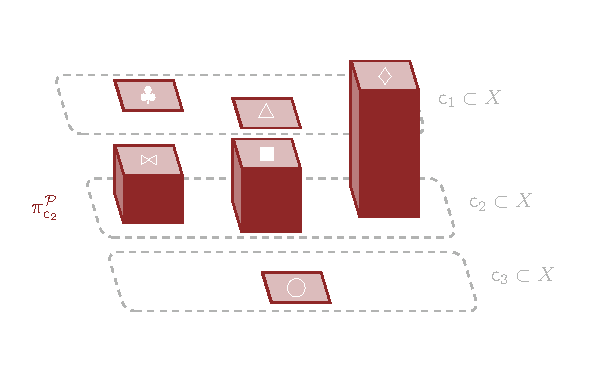
\includegraphics{figures/conditional_distribution/ambient/ambient.pdf}

}

\subcaption{\label{fig-conditional-interpretations-ambient}}

\end{minipage}%
%
\begin{minipage}{0.50\linewidth}

\centering{

\captionsetup{labelsep=none}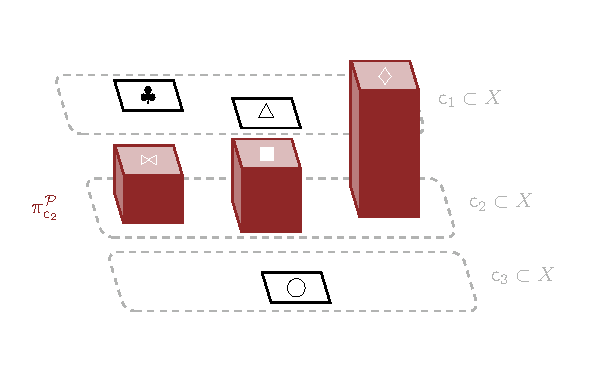
\includegraphics{figures/conditional_distribution/restricted/restricted.pdf}

}

\subcaption{\label{fig-conditional-interpretations-restricted}}

\end{minipage}%

\caption{\label{fig-conditional-interpretations}Conditional probability
distributions can be interpreted in two equally valid ways. (a) We can
interpret a conditional probability distribution as a probability
distribution over the entire space which concentrates all of its
probability into to a single partition cell. Here
\(\pi^{\mathcal{P}}_{ \mathsf{c}_{2} }\) allocates non-zero probability
to only the elements of the partition cell
\(\mathsf{c}_{2} = \{ \blacksquare, \diamondsuit, \bowtie \}\). (b)
Alternatively we can interpret a conditional probability distribution as
a probability distribution defined over a single partition cell. From
this perspective \(\pi^{\mathcal{P}}_{ \mathsf{c}_{2} }\) doesn't even
consider elements outside of \(\mathsf{c}_{2}\).}

\end{figure}%

The former interpretation is more common in technical mathematics. As we
will see later on in this chapter and the next, however, the latter
interpretation is more in line with how conditional probability
distributions work are interpreted and used in more practical
applications of probability theory.

\subsection{Conditional Probability
Kernels}\label{conditional-probability-kernels}

We can push our organization one step further and collect all of the
conditional probability distributions for all of the partition cells
into a single mathematical object
(Figure~\ref{fig-conditional-organization}) \begin{alignat*}{6}
\pi^{\mathcal{P}}( \cdot \mid \cdot )
:\; &\mathcal{X} \times \mathcal{P}& &\rightarrow& \; &[0, 1]&
\\
&\mathsf{x}, \mathsf{c}& &\mapsto&
&\frac{ \pi(\mathsf{x} \cap \mathsf{c}) }{ \pi (\mathsf{c}) }&.
\end{alignat*} I will refer to this binary function as a
\textbf{conditional probability kernel}.

\begin{figure}

\begin{minipage}{0.05\linewidth}
~\end{minipage}%
%
\begin{minipage}{0.30\linewidth}

\centering{

\captionsetup{labelsep=none}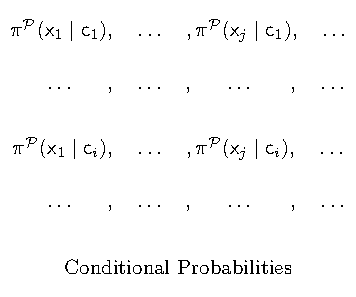
\includegraphics{figures/conditional_distribution/organization/probabilities/probabilities.pdf}

}

\subcaption{\label{fig-conditional-organization-probabilities}}

\end{minipage}%
%
\begin{minipage}{0.30\linewidth}

\centering{

\captionsetup{labelsep=none}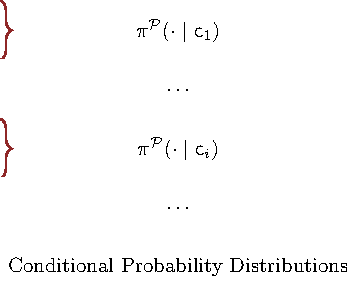
\includegraphics{figures/conditional_distribution/organization/distributions/distributions.pdf}

}

\subcaption{\label{fig-conditional-organization-distributions}}

\end{minipage}%
%
\begin{minipage}{0.30\linewidth}

\centering{

\captionsetup{labelsep=none}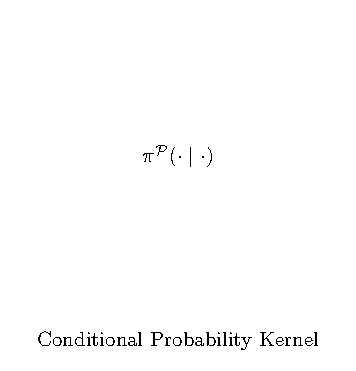
\includegraphics{figures/conditional_distribution/organization/kernel/kernel.pdf}

}

\subcaption{\label{fig-conditional-organization-kernel}}

\end{minipage}%
%
\begin{minipage}{0.05\linewidth}
~\end{minipage}%

\caption{\label{fig-conditional-organization}An important part of
conditional probability theory is organization. (a) The conditional
probabilities defined by \(\pi\)-non-null partition cells can be
organized into (b) conditional probability distributions that return
conditional probabilities when evaluated. Likewise the collection of
conditonal probability distributions defined by all partition cells can
be organized into a conditional probability kernel that returns
conditonal probability distributions when partially evaluated. In order
to generalize conditional probability theory to \(\pi\)-null partitions
we will actually work backwards, showing first that a conditional
probability kernel exists and then deriving conditonal probability
distributions from the kernel and conditional probabilities from those
distributions.}

\end{figure}%

Partially evaluating a conditional probability kernel on a measurable
subset in its first argument results in a measurable, unary function
from each partition cell to the corresponding conditional probability,
\begin{alignat*}{6}
p_{\mathsf{x}}
=
\pi^{\mathcal{P}}( \mathsf{x} \mid \cdot )
:\; &\mathcal{P}& &\rightarrow& \; &[0, 1]&
\\
&\mathsf{c}& &\mapsto&
&\frac{ \pi(\mathsf{x} \cap \mathsf{c}) }{ \pi (\mathsf{c}) }&.
\end{alignat*} In words this partial evaluation quantifies how much the
unconditional probability allocated to \(\mathsf{x}\) contributes to the
unconditional probability allocated to each partition cell. I will refer
to this object as a \textbf{conditional probability function}.

On the other hand partially evaluating a conditional probability kernel
on a partition cell in its second argument gives the corresponding
conditional probability distribution, \begin{alignat*}{6}
\pi^{\mathcal{P}}_{\mathsf{c}}
=
\pi^{\mathcal{P}}( \cdot \mid \mathsf{c} )
:\; &\mathcal{X}& &\rightarrow& \; &[0, 1]&
\\
&\mathsf{x}& &\mapsto&
&\frac{ \pi(\mathsf{x} \cap \mathsf{c}) }{ \pi (\mathsf{c}) }&.
\end{alignat*}

As is so often the case we have to be careful with the terminology here.
I have used ``conditional probability distribution'' to refer to a
particular probability distribution associated with a particular
partition cell, and ``conditional probability kernel'' to refer to the
collection of all probability distributions defined by all of the cells
in a partition.

This convention, however, is by no means universal. Many references use
``conditional probability distribution'' to refer to the collection of
probability distributions \(\pi^{\mathcal{P}}\) instead of a particular
probability distribution \(\pi^{\mathcal{P}}_{\mathsf{c}}\), and some
even use it to refer to both at the same time! Needless to say this
latter overloaded and ambiguous terminology makes it very easy to
confuse the two objects.

Again I will use ``conditional probability distribution'' and
``conditional probability kernel'' to avoid as much ambiguity in this
book as possible, but when reading other texts you may want to be
careful to identify to which object an author is referring as any given
time. Moreover in our own writing there is no harm in being redundant in
order clarify whether we are referring to
\(\pi^{\mathcal{P}}( \cdot \mid \cdot )\) or
\(\pi^{\mathcal{P}}( \cdot \mid \mathsf{c} )\) in any given application.

\subsection{The Law of Total
Expectation}\label{the-law-of-total-expectation}

One of the benefits of conditional probability kernels is that they
allow us to rewrite the law of total probability, \[
\pi( \mathsf{x} )
=
\sum_{ \mathsf{c} \in \mathcal{P} }
\pi^{\mathcal{P}}( \mathsf{x} \mid \mathsf{c} ) \, \pi( \mathsf{c} )
\] entirely in terms of expectation values.

If we write conditional probabilities as the outputs of a conditional
probability function function, \[
\pi^{\mathcal{P}}( \mathsf{x} \mid \mathsf{c} )
=
p_{\mathsf{x}}( \mathsf{c} ),
\] then the law of total probability becomes a discrete expectation
value, \begin{align*}
\pi( \mathsf{x} )
&=
\sum_{ \mathsf{c} \in \mathcal{P} }
\pi^{\mathcal{P}}( \mathsf{x} \mid \mathsf{c} ) \, \pi( \mathsf{c} )
\\
&=
\sum_{ \mathsf{c} \in \mathcal{P} }
p_{\mathsf{x}}( \mathsf{c} ) \, \pi( \mathsf{c} )
\\
&=
\mathbb{E}_{ \pi_{\mathcal{P}} } [ p_{\mathsf{x}} ].
\end{align*} Here the probability distribution \(\pi_{\mathcal{P}}\) is
defined by the probability allocated to each partition cell, \[
\pi_{\mathcal{P}}( \mathsf{c} ) = \pi( \mathsf{c} ).
\]

At the same time both the initial allocation and conditional probability
function can be written in terms of expectation values of indicator
functions, \[
\pi( \mathsf{x} )
=
\mathbb{E}_{\pi}[ I_{\mathsf{x}} ]
\] and \[
p_{\mathsf{x}}(\mathsf{c})
=
\mathbb{E}_{\pi^{\mathcal{P}}_{\mathsf{c}} }[ I_{\mathsf{x}} ],
\] respectively. Consequently we can write the law of total probability
as \begin{align*}
\pi( \mathsf{x} )
&=
\mathbb{E}_{ \pi_{\mathcal{P}} } [ p_{\mathsf{x}} ]
\\
\mathbb{E}_{\pi}[ I_{\mathsf{x}} ]
&=
\mathbb{E}_{ \pi_{\mathcal{P}} } [ p_{\mathsf{x}} ]
\end{align*} with \[
p_{\mathsf{x}}(\mathsf{c})
=
\mathbb{E}_{\pi^{\mathcal{P}}_{\mathsf{c}} }[ I_{\mathsf{x}} ].
\]

Conveniently this relationship between the various notions of
expectation defined by an initial probability distribution \(\pi\) and a
measurable partition \(\mathcal{P}\) generalizes to arbitrary
expectation values. The expectation value of \emph{any} function \[
g : (X, \mathcal{X}) \rightarrow
    (\mathbb{R}, \mathcal{B}_{\mathbb{R}})
\] can be written as \[
\mathbb{E}_{\pi}[ g ]
=
\mathbb{E}_{ \pi_{\mathcal{P}} } [ e_{g} ],
\] where \[
e_{g}(\mathsf{c})
=
\mathbb{E}_{ \pi^{\mathcal{P}}_{\mathsf{c}} }[ g ].
\] Here the inner expectations \(e_{g}\) are known as
\textbf{conditional expectation values} and the overall result is known
as the \textbf{law of total expectation} or the \textbf{law of iterated
expectation}.

With the laws of total probability and total expectation in hand we can
decompose not only probability allocations but also expectation values
along an explicit partition. If expectation values with respect to the
initial probability distribution are difficult to compute but the
conditional expectation values are more straightforward to work out then
this iterative approach becomes a particularly-productive computational
technique.

\section{Conditioning On Implicit
Partitions}\label{conditioning-on-implicit-partitions}

The construction, and notation, of conditional probability distributions
becomes particularly elegant when we implicitly define countable
partitions through the level sets of a surjective function. This also
paves the way for generalizing conditional probability theory to
uncountable partitions implicitly defined by functions with an
uncountable number of output points.

\subsection{Conditioning On Countable Implicit
Partitions}\label{conditioning-on-countable-implicit-partitions}

In \hyperref[sec:partitions]{Section 1} we learned that surjective
functions \(f : X \rightarrow Y\) implicitly define a partition of the
input space \(X\) where the partition cells are defined by the non-empty
level sets \(f^{-1}(y) \subset X\). If \(f\) is also
\((\mathcal{X}, \mathcal{Y})\)-measurable and \(\mathcal{Y}\) is a
Hausdorff \(\sigma\)-algebra then these non-empty level sets will also
be \(\mathcal{X}\) measurable, allowing us to consistently allocate
probability to them.

When \(Y\) contains a countable number of elements the partition defined
by these level sets will be countable. Moreover if the probability
allocated to each level set is non-zero, \[
\pi( f^{-1}(y) ) > 0
\] for all \(y \in Y\), then the partition will be \(\pi\)-non-null. In
this case we can directly apply the conditional probability theory that
we introduced in \hyperref[sec:explicit-conditional]{Section 2}.

When working with partitions implicitly defined by a surjective function
\(f : (X, \mathcal{X}) \rightarrow (Y, \mathcal{Y})\) I will denote the
conditional probability kernel as \begin{alignat*}{6}
\pi^{f} :\; &\mathcal{X} \times Y& &\rightarrow& \; &[0, 1]&
\\
&\mathsf{x}, y& &\mapsto&
&\pi^{f} ( \mathsf{x} \mid y ) =
 \frac{ \pi(\mathsf{x} \cap f^{-1}(y)) }{ \pi(f^{-1}(y)) } &.
\end{alignat*}

For each \(\mathsf{x} \in \mathcal{X}\) the partial evaluation \[
p_{\mathsf{x}} = \pi^{f} ( \mathsf{x} \mid \cdot )
: Y \rightarrow [0, 1]
\] defines a \(\mathcal{Y}\)-measurable conditional probability
function, and for each \(y \in Y\) the partial evaluation
\begin{alignat*}{6}
\pi^{f}_{y} = \pi^{f} ( \cdot \mid y )
:\; &\mathcal{X}& &\rightarrow& \; &[0, 1]&
\\
&\mathsf{x}& &\mapsto& &\pi^{f} ( \mathsf{x} \mid y )  &
\end{alignat*} defines a conditional probability distribution that
concentrates entirely on the corresponding level set, \begin{align*}
\pi^{f}_{y}( f^{-1}(y) )
&=
\pi^{f}( f^{-1}(y) \mid y )
\\
&=
\frac{ \pi(f^{-1}(y) \cap f^{-1}(y)) }{ \pi(f^{-1}(y)) }
\\
&=
\frac{ \pi(f^{-1}(y) ) }{ \pi(f^{-1}(y)) }
\\
&=
1.
\end{align*}

Equivalently we can interpret each \(\pi^{f}_{y}\) as a probability
distribution over not the entire ambient space \(X\) but rather just the
corresponding level set, \[
\pi^{f}_{y} : \mathcal{X}_{y} \rightarrow [0, 1],
\] where \(\mathcal{X}_{y}\) denotes the subspace \(\sigma\)-algebra
restricted to the level set \(f^{-1}(y)\). Again we have the flexibility
to interpret the conditional probability distributions induced by \(f\)
as a collection of probability distributions over \(X\) that concentrate
on particular level sets or as a collection of probability distributions
over the particular level sets themselves.

At the same time because we have assumed that \(f\) is
\((\mathcal{X}, \mathcal{Y})\)-measurable we can push \(\pi\) forward
along \(f\) to define a marginal probability distribution \(f_{*} \pi\)
over the output space. By definition the pushforward probability
allocated to the output atomic subset \(\{ y \} \in \mathcal{Y}\) is
equal to the input probability allocated to the corresponding level set,
\[
f_{*} \pi( \{ y \} ) = \pi ( f^{-1}(y) ).
\] This means that a surjective function
\(f : (X, \mathcal{X}) \rightarrow (Y, \mathcal{Y})\) induces a
\(\pi\)-non null partition if and only if the pushforward probability
allocated to every output atomic subset is non-zero, \[
f_{*} \pi( \{ y \} ) > 0
\] for all \(y \in Y\).

For the countable and measurable partition implicitly defined by a
sufficiently nice surjective function the law of total probability
becomes \begin{align*}
\pi( \mathsf{x} )
&=
\sum_{ y \in Y }
\pi^{f}( \mathsf{x} \mid y ) \, \pi(f^{-1}(y))
\\
&=
\sum_{ y \in Y }
\pi^{f}( \mathsf{x} \mid y ) \, f_{*} \pi( \{ y \} ).
\end{align*} This, however, is just a pushforward expectation value,
\begin{align*}
\pi( \mathsf{x} )
&=
\sum_{ y \in Y }
\pi^{f}( \mathsf{x} \mid y ) \, f_{*} \pi( \{ y \} )
\\
&=
\mathbb{E}_{f_{*}\pi} [ p_{\mathsf{x}} ],
\end{align*} where \begin{alignat*}{6}
p_{\mathsf{x}} :\; &Y& &\rightarrow& \; &[0, 1]&
\\
&y& &\mapsto& &\pi^{f}( \mathsf{x} \mid y ) =
\frac{ \pi(\mathsf{x} \cap f^{-1}(y)) }{ \pi(f^{-1}(y)) }&
\end{alignat*} is just a conditional probability function.

Similarly the law of total expectation becomes \begin{align*}
\mathbb{E}_{\pi}[ g ]
&=
\sum_{ x \in X } \pi( \{ x \} ) \, g(x)
\\
&=
\sum_{ x \in X }
\left[ \sum_{ y \in Y }
\pi^{f}( \{ x \} \mid y ) \, f_{*} \pi( \{ y \} )
\right] \, g(x)
\\
&=
\sum_{ y \in Y }
\left[
\sum_{ x \in X }
\pi^{f}( \{ x \} \mid y ) \, g(x)
\right] \, f_{*} \pi( \{ y \} )
\\
&=
\sum_{ y \in Y }
e_{g} \, f_{*} \pi( \{ y \} )
\\
&=
\mathbb{E}_{ f_{*} \pi } [ e_{g} ],
\end{align*} where \(e_{g}\) is the conditional expectation function
\begin{alignat*}{6}
e_{g} :\; &Y& &\rightarrow& \; &[0, 1]&
\\
&y& &\mapsto& & \mathbb{E}_{\pi^{f}_{y} }[ g ] &.
\end{alignat*}

Notice that a sufficiently-nice surjective function gives us two ways to
manipulate a probability distribution over the input space: we can not
only push it forward to a probability distribution on the output space
but also decompose it into a collection of probability distributions
across the level sets. Moreover the laws of total probability and total
expectation show us that these operations complement each other in the
sense that we can always recover any information about the initial
probability distribution by combining the information from the
pushforward and conditional probability distributions.

In other words conditional probability distributions encodes all of the
information that we might lose when pushing a probability distribution
forward along a surjective function. The pushforward probability
distribution quantifies how much input probability is allocated to each
level set while each conditional probability distribution quantifies how
those allocations are distributed all across the corresponding level set
(Figure~\ref{fig-implicit-decomposition}).

\begin{figure}

\begin{minipage}{0.66\linewidth}

\centering{

\captionsetup{labelsep=none}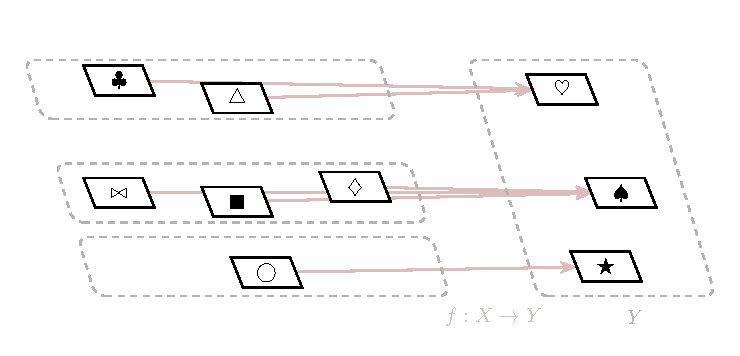
\includegraphics{figures/decomposition/function/function.pdf}

}

\subcaption{\label{fig-decomposition-function}}

\end{minipage}%
%
\begin{minipage}{0.34\linewidth}

\centering{

\captionsetup{labelsep=none}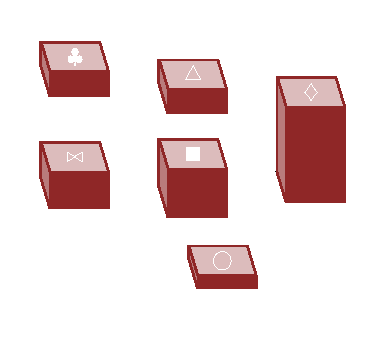
\includegraphics{figures/decomposition/initial/initial.pdf}

}

\subcaption{\label{fig-decomposition-function}}

\end{minipage}%
\newline
\begin{minipage}{0.17\linewidth}

\centering{

\captionsetup{labelsep=none}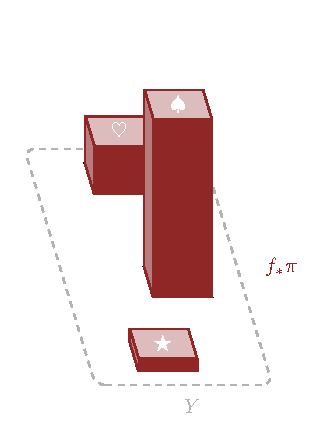
\includegraphics{figures/decomposition/marginal/marginal.pdf}

}

\subcaption{\label{fig-decomposition-function}}

\end{minipage}%
%
\begin{minipage}{0.83\linewidth}

\centering{

\captionsetup{labelsep=none}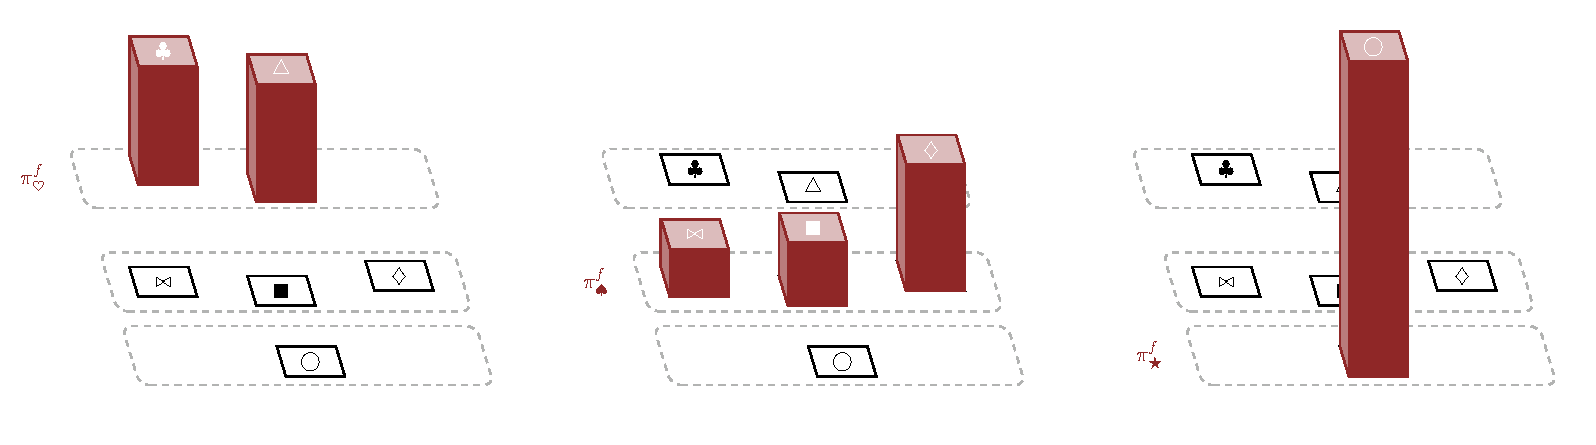
\includegraphics{figures/decomposition/conditional/conditional.pdf}

}

\subcaption{\label{fig-decomposition-function}}

\end{minipage}%

\caption{\label{fig-implicit-decomposition}The partition implicitly
defined by a surjective function can also be used to condition. (a) The
level sets (b) decompose an initial probability distribution into (c) a
pushforward probability distribution and (d) a conditional probability
kernel. All of the information in the initial probability distribution
is preserved one of these components. Moreover all probabilistic
operations defined by the initial probability distribution can be
computed using the pushforward and conditional probability distributions
with the law of total expectation.}

\end{figure}%

Conditioning on implicit conditions suggests a variety of terminologies.
We might, for example, say that we're conditioning the initial
probability distribution \(\pi\) on a surjective function
\(f : X \rightarrow Y\), the output points \(y \in Y\), the level sets
defined by that point \(f^{-1}(y) \in Y\), or even the subspace
\(\sigma\)-algebras within that level set. All of this language,
however, is just short-hand for conditioning on the \emph{partition}
implied by all of these intermediate objects.

\subsection{Conditioning On General Implicit
Partitions}\label{sec:general-conditional}

Up to this point we have been able to define conditional probability
distributions for measurable, \(\pi\)-non-null, and countable partitions
that are defined either explicitly as a list of subsets or implicitly as
the level sets of a surjective function. Unfortunately this construction
doesn't immediately generalize to the continuous spaces that dominate
practical applications.

Consider for example a surjective function
\(f: (X, \mathcal{X}) \rightarrow (Y, \mathcal{Y})\) where both the
input space \(X\) and output space \(Y\) are continuous spaces with an
uncountably infinite number of elements. This function implicitly
defines a partition of the input space \(X\) into an uncountably
infinite number of level sets \(f^{-1}(y)\).

As in the countable case we can decompose any measurable subset
\(\mathsf{x} \in \mathcal{X}\) into its intersections with these level
sets (Figure~\ref{fig-general-decomposition}), \[
\mathsf{x} = \bigcup_{y \in Y} \left( \mathsf{x} \cap f^{-1}(y) \right).
\] Because there are an uncountably infinite number of intersections,
however, we cannot write \(\pi(\mathsf{x})\) as a sum over the
intersection probabilities, \[
\pi( \mathsf{x} )
=
\pi \left( \bigcup_{y \in Y}
           \left( \mathsf{x} \cap f^{-1}(y) \right) \right)
\ne
\sum_{y \in Y} \pi( \mathsf{x} \cap f^{-1}(y) ).
\] Remember that probability distributions are defined to have
\emph{countable} additivity but not uncountable additivity! Consequently
we cannot define a law of total probability as a sum over individual
output elements.

\begin{figure}

\begin{minipage}{0.50\linewidth}

\centering{

\captionsetup{labelsep=none}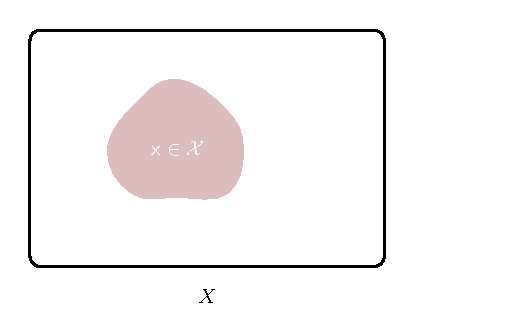
\includegraphics{figures/decomposition/continuous/subset/subset.pdf}

}

\subcaption{\label{fig-decomposition-subset}}

\end{minipage}%
%
\begin{minipage}{0.50\linewidth}

\centering{

\captionsetup{labelsep=none}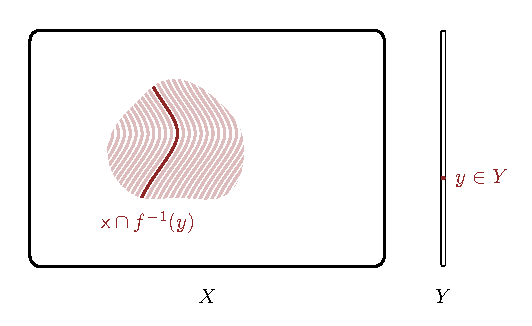
\includegraphics{figures/decomposition/continuous/decomposition/decomposition.pdf}

}

\subcaption{\label{fig-decomposition-continuous}}

\end{minipage}%

\caption{\label{fig-general-decomposition}Given an uncountable partition
(a) any measurable subset set (b) can be decomposed into an uncountable
number of level set intersections. Because probability distributions are
required to be only countably additive we cannot distribution
probability allocations through this decomposition.}

\end{figure}%

At the same time many probability distributions that we will encounter
in practical applications of probability theory will allocate zero
probability to either some or all of the level sets of the conditioning
function, \[
\pi(f^{-1}(y))
= f_{*} \pi( \{ y \} )
= 0.
\] Consequently any attempt to directly define general conditional
probabilities by the ratio \[
\pi^{f}( \mathsf{x} \mid y )
=
\pi^{f}_{y}( \mathsf{x} )
=
\frac{ \pi( \mathsf{x} \cap f^{-1}(y) ) }{ \pi( f^{-1}(y) ) }
\] would result with indefinite \(0 / 0\) outcomes.

Is there any hope for generalizing conditional probability to
uncountable partitions? Fortunately the answer is yes. While we cannot
\emph{sum} over the individual level set probabilities we can define
\emph{expectations} over them. In particular the key is to generalize
the expectation form of the law of total probability, \[
\pi( \mathsf{x} )
=
\mathbb{E}_{f_{*}\pi} [ p_{\mathsf{x}} ],
\] for some appropriate function \[
p_{\mathsf{x}} : Y \rightarrow [0, 1]
\] that we will have to define. Equivalently we can generalize the law
of total expectation, \[
\mathbb{E}_{\pi}[ g ]
=
\mathbb{E}_{ f_{*} \pi } [ e_{g} ],
\] for some appropriate function \[
e_{g} : Y \rightarrow [0, 1].
\]

To formalize this generalization consider a surjective function
\(f : (X, \mathcal{X}) \rightarrow (Y, \mathcal{Y})\) and a probability
distribution \(\pi : \mathcal{X} \rightarrow [0, 1]\). An intricate
mathematical analysis (Chang and Pollard (1997); Leão Jr, Fragoso, and
Ruffino (2004)) shows that if \(\pi\) is sufficiently well-behaved then,
in addition to the pushforward distribution \[
f_{*} \pi : \mathcal{Y} \rightarrow [0, 1],
\] there always exists a conditional probability kernel
\begin{alignat*}{6}
\pi^{f} ( \cdot \mid \cdot )
:\; &\mathcal{X} \times Y& &\rightarrow& \; &[0, 1] \subset \mathbb{R}&
\\
&\mathsf{x}, y& &\mapsto& &\pi^{f} ( \mathsf{x} \mid y )&,
\end{alignat*} that gives a
\((\mathcal{Y}, \mathcal{B}_{\mathbb{R}})\)-measurable conditional
probability function for any partial evaluation on the first argument,
\[
\pi^{f} ( \mathsf{x} \mid \cdot ) : Y \rightarrow [0, 1],
\] and a conditional probability distribution for \(f_{*} \pi\)-almost
every partial evaluation on the second argument, \begin{alignat*}{6}
\pi^{f}_{y}
:\; &\mathcal{X}& &\rightarrow& \; &[0, 1]&
\\
&\mathsf{x}& &\mapsto& &\pi^{f} ( \mathcal{x} \mid y ) &.
\end{alignat*} In particular the conditional probability distributions
concentrate on the corresponding level set, \[
\pi^{f}_{y}( f^{-1}(y) ) = \pi^{f}( f^{-1}(y) \mid y ) = 1,
\] just as in the countable case.

Critically these partial evaluations satisfy a generalized law of total
probability (Figure~\ref{fig-general-total-probability}), \[
\pi( \mathsf{x} ) = \mathbb{E}_{f_{*} \pi} [ p_{\mathsf{x}} ]
\] where \(p_{\mathsf{x}}(y)\) is the conditional probability function.
Moreover they also satisfy a generalized law of total expectation, \[
\mathbb{E}_{\pi}[g]
=
\mathbb{E}_{f_{*} \pi} [ e_{g} ]
\] where \begin{alignat*}{6}
e_{g} :\; &Y& &\rightarrow& \; &[0, 1]&
\\
&y& &\mapsto& &\mathbb{E}_{\pi^{f}_{y} }[ g ] &
\end{alignat*} is a conditional expectation value.

\begin{figure}

\centering{

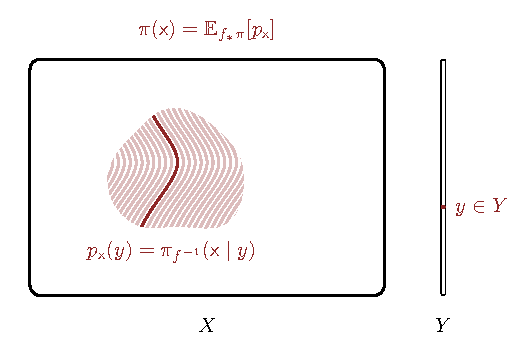
\includegraphics[width=0.5\textwidth,height=\textheight]{figures/total_probability/general/general.pdf}

}

\caption{\label{fig-general-total-probability}Although we can't always
sum over the probabilities allocated to the intersection of a measurable
subset \(\mathsf{x} \in \mathcal{X}\) with the level sets of a
sufficiently well-behaved function, we can take a pushforward
expectation over the relative level set probabilities,
\(\pi(\mathsf{x}) = \mathbb{E}_{f_{*} \pi} [ p_{\mathsf{x}}]\).}

\end{figure}%

In the case where the output space, and hence the number of level sets,
is countable these expectations reduce to discrete summations, and the
general laws of total probability and expectation reduce to our initial
laws of total probability and expectation. For example \begin{align*}
\pi( \mathsf{x} )
&=
\mathbb{E}_{f_{*} \pi} [ p_{\mathsf{x}} ]
\\
&=
\sum_{y \in Y} f_{*} \pi(y) \, p_{\mathsf{x}}(y)
\\
&=
\sum_{y \in Y} \pi( f^{-1}( \{ y \} ) ) \, p^{f^{-1}}(\mathsf{x} \mid y)
\\
&=
\sum_{y \in Y} \pi( f^{-1}( \{ y \} ) ) \,
\frac{ \pi( \mathsf{x} \cap f^{-1}( \{ y \} ) )}
{ \pi( f^{-1}( \{ y \} ) ) }.
\end{align*}

Any conditional probability kernel satisfying these properties is
referred to as a \textbf{disintegration} of the probability distribution
\(\pi\) with respect to \(f\) or, far less impressively, a
\textbf{regular conditional probability distribution}, or
\textbf{regular conditional probability kernel}. That said I find names
like ``regular conditional probability kernel'' to be a bit of a
mouthful. To streamline the terminology slightly I will use
``conditional probability kernel'' to refer to disintegrations
generally, and ``discrete conditional probability kernel'' to refer to
the special case of disintegrations with respect to functions that
implicitly define countable partitions.

For countable output spaces a surjective function \(f\) and probability
distribution \(\pi\) uniquely define a disintegration, and hence a
discrete conditional probability kernel. More generally there will be
infinitely many disintegrations compatible with a given function and
probability distribution pair. The differences between these compatible
disintegrations, however, are always confined to \(\pi\)-null subsets
and, consequently, they all define equivalent probabilities and
expectation values.

Disintegrations completely generalize the discrete conditional
probability kernels that we derived for countable partitions. We can
interpret disintegrations as a collection of probability distributions
that concentrate on particular level sets or, equivalently, a collection
of probability distributions defined directly on particular level sets.
Moreover disintegrations can be also be interpreted as complementing the
pushforward probability distribution, with the latter determining how
much probability is allocated to each level set and the former
determining how that total allocation unfurls across each level set.

There is one final technical detail that I have purposefully left
ambiguous. Earlier I noted that disintegrations exist not for any
probability distribution but rather only sufficiently ``well-behaved''
probability distributions. For those interested in exploring these
details disintegrations can be derived only for a special class of
measures known as \textbf{Radon measures}. Understanding what Radon
measures are, and why they are needed to define disintegrations, goes
far beyond the scope of this book. Fortunately every probability
distribution we will encounter will be a Radon probability distribution,
indeed non-Radon probability distributions are extremely weird
mathematically, and we can consequently take this condition for granted.

\section{Conditional Probability Density
Functions}\label{conditional-probability-density-functions}

Conditional probability distributions are relatively straightforward to
define abstractly. In practice, however, we will typically be working
with not these probability distributions directly but rather their
probability density function representations in the context of a
convenient reference measure.

Unfortunately rigorously constructing conditional probability density
functions is a bit more complicated. To do so properly we will need
\emph{all} of the measure theory tools that we have developed to this
point, and a few more that I will introduce below. Buckle up and make
sure that you are aware of for your nearest emergency exit.

\subsection{The Utility Of Integral
Notation}\label{the-utility-of-integral-notation}

Before diving into probability density functions let's take a second to
ponder notation.

Recall that partially evaluating a regular conditional probability
kernel on any \(y \in Y\) yields a conditional probability distribution
that concentrates on the level set \(f^{-1}(y)\), \begin{alignat*}{6}
\pi^{f}_{y} :\; &\mathcal{X}& &\rightarrow& \; &[0, 1]&
\\
&\mathsf{x}& &\mapsto& &\pi^{f}( \mathsf{x} \mid y )&.
\end{alignat*} When paired with an integrand
\(g : X \rightarrow \mathbb{R}\) the collection of all conditional
probability distributions then defines a conditional expectation
function, \begin{alignat*}{6}
e_{g} : \; &Y& &\rightarrow& \; &\mathbb{R}&
\\
&y& &\mapsto& & \mathbb{E}_{ \pi^{f}_{y} } \! \left[  g  \right]&.
\end{alignat*} The law of total expectation ensures that the pushforward
expectation of this conditional expectation function is always equal to
the expectation value of the probability distribution that was
disintegrated, \[
\mathbb{E}_{\pi} \! \left[ g \right] = \mathbb{E}_{ f_{*} \pi } \! \left[ e_{g} \right].
\]

Ideally we'd be able to write the law of total expectation more
compactly, packing all of the contributions into a single line.
Unfortunately any attempt at more compact notation is frustrated by the
standard notational convention of ignoring arguments when denoting
expectation values.

For example a notation that replaces \(y\) with a placeholder
``\(\cdot\)'', \[
\mathbb{E}_{\pi} \! \left[ g \right]
= \mathbb{E}_{ f_{*} \pi } \! \left[ e_{g} \right]
= \mathbb{E}_{ f_{*} \pi } \! \left[  \mathbb{E}_{\pi^{f}_{\cdot}} \! \left[ g \right]  \right],
\] is not only hard to read but can be ambiguous in applications where
there are multiple spaces on which \(f\) and \(g\) might act. At the
same time a notation like \[
\mathbb{E}_{\pi} \! \left[ g \right]
= \mathbb{E}_{ f_{*} \pi } \! \left[ e_{g} \right]
= \mathbb{E}_{ f_{*} \pi } \! \left[  \mathbb{E}_{\pi^{f}_{y}} \! \left[ g(x) \right]  \right]
\] fails to communicate on what spaces the probability distributions
\(f_{*} \pi\) and \(\pi^{f}_{y}\) are defined.

One way around these notational frustrations is to use the integral
notation for expectation values that we first discussed in
\href{https://betanalpha.github.io/assets/chapters_html/expectation_values.html\#sec:alt_notations}{Chapter
5, Section 2.4} where appropriate variables specify the spaces on which
all of the probability distributions and functions are defined.

For example if we interpret each conditional probability distribution
\(\pi^{f}_{y}\) as being defined over the entirely of the ambient space
\(X\) then the conditional expectation function can be written as
\begin{align*}
e_{g}(y)
&=
\mathbb{E}_{ \pi^{f}_{y} } \! \left[  g  \right]
\\
&=
\int \pi^{f}( \mathrm{d} x \mid y ) \, g(x),
\end{align*} with the law of total expectation nesting measure-informed
integrals over the entire ambient space within measure-informed
integrals over the output space, \begin{align*}
\mathbb{E}_{\pi} \! \left[ g \right]
&=
\mathbb{E}_{ f_{*} \pi } \! \left[ e_{g} \right]
\\
\int \pi( \mathrm{d} x ) \, g(x)
&=
\int f_{*} \pi (\mathrm{d} y) \, e_{g}(y)
\\
\int \pi( \mathrm{d} x ) \, g(x)
&=
\int f_{*} \pi (\mathrm{d} y)
\int \pi^{f}_{y}( \mathrm{d} x) \, g(x)
\\
\int \pi( \mathrm{d} x ) \, g(x)
&=
\int f_{*} \pi (\mathrm{d} y)
\int \pi^{f}( \mathrm{d} x \mid y ) \, g(x).
\end{align*}

To use the integral notation when we interpret each conditional
probability distribution \(\pi^{f}_{y}\) as being defined over only the
corresponding level set \(f^{-1}(y) \subset X\) we need to be able to
specify variables that take values in that level set. To that end let's
introduce a \textbf{conditional variable} \(x_{y}\) that takes values in
the level set corresponding to the output point \(y \in Y\), \[
x_{y} \in f^{-1}(y) \subset X.
\] Conditional variables allow us to decompose any input variable
\(x \in X\) into an output variable and a corresponding conditional
variable, \[
x = (y, x_{y}).
\] Note that the right hand-side isn't an ordered pair because the
possible values of the second variable will in general depend on the
choice of the first variable. For the mathematically-curious this
construction is known as a \textbf{semi-direct product}.

Using conditional variables we can then write the conditional
expectation function as \begin{align*}
e_{g}(y)
&=
\mathbb{E}_{ \pi^{f}_{y} } \! \left[  g  \right]
\\
&=
\int \pi^{f}_{y}( \mathrm{d} x_{y} ) \, g(y, x_{y})
\\
&=
\int \pi^{f}( \mathrm{d} x_{y} \mid y ) \, g(y, x_{y}).
\end{align*} The law of total expectation then nests measure-informed
integrals over the level sets of \(f\) within an measure-informed
integral over the output space, \begin{align*}
\mathbb{E}_{\pi} \! \left[ g \right]
&=
\mathbb{E}_{ f_{*} \pi } \! \left[ e_{g} \right]
\\
\int \pi( \mathrm{d} x ) \, g(x)
&=
\int f_{*} \pi (\mathrm{d} y) \, e_{g}(y)
\\
\int \pi( \mathrm{d} x ) \, g(x)
&=
\int f_{*} \pi (\mathrm{d} y)
\int \pi^{f}( \mathrm{d} x_{y} \mid y ) \, g(y, x_{y}).
\end{align*}

Conditional variables are by no means universal and there many other
notational conventions for specifying measure-informed integrals over
individual level sets that one might encounter. Some references, for
example, decorate the integral sign with the relevant spaces, \[
\int_{X} \pi( \mathrm{d} x ) \, g(x)
=
\int_{Y} f_{*} \pi (\mathrm{d} y)
\int_{f^{-1}(y)} \pi^{f}( \mathrm{d} x \mid y ) \, g(x),
\] while others use \(\delta\) function-like shorthands such as \[
\int \pi( \mathrm{d} x ) \, g(x)
=
\int f_{*} \pi (\mathrm{d} y)
\int \pi^{f}( \mathrm{d} x \mid y ) \, \delta(y - f(x)) \, g(x)
\] or \[
\int \pi( \mathrm{d} x ) \, g(x)
=
\int f_{*} \pi (\mathrm{d} y)
\int \pi^{f}( \mathrm{d} x \mid y ) \, \delta(f^{-1}(y)) \, g(x)
\] to communicate the domain of integration. In this book, however, I
will tend to favor the conditional variable notation as I find that it
offers the best compromise between compactness and informativeness.

Finally the integral relationships implied by the law of total
expectation are often simplified to relationships between the
integrands. For example \[
\int \pi( \mathrm{d} x ) \, g(x)
=
\int f_{*} \pi (\mathrm{d} y)
\int \pi^{f}( \mathrm{d} x \mid y ) \, g(x)
\] might be represented by \[
\pi( \mathrm{d} x )
=
f_{*} \pi (\mathrm{d} y) \pi^{f}( \mathrm{d} x \mid y ),
\] and \[
\int \pi( \mathrm{d} x ) \, g(x)
=
\int f_{*} \pi (\mathrm{d} y)
\int \pi^{f}( \mathrm{d} x_{y} \mid y ) \, g(x_{y})
\] represented by \[
\pi( \mathrm{d} x )
=
f_{*} \pi (\mathrm{d} y) \pi^{f}( \mathrm{d} x_{y} \mid y ).
\]

We always have to be careful, however, to recognize that these simpler
integrand equations are just notational shorthands for the full integral
relationships and not misinterpret them otherwise. For example in
general we do not have \[
\pi( \mathsf{x} )
=
f_{*} \pi (\mathsf{y}) \pi^{f}( \mathsf{x} \mid y )
\] for any combination of input subset \(\mathsf{x} \in \mathcal{X}\),
output subset \(\mathsf{y} \in \mathcal{Y}\), and output point
\(y \in Y\).

\subsection{Conditional Probability Density Functions For Non-Null
Partitions}\label{sec:discrete-conditional-density}

With our notational tools set let's make our first step into conditional
probability density functions by considering the simplest case of a
countable, non-null partition.

As usual we begin with an initial probability space
\((X, \mathcal{X}, \pi)\). Next we'll introduce a surjective function
\(f : (X, \mathcal{X}) \rightarrow (Y, \mathcal{Y})\) that maps the
initial space into a countable output space such that each level set is
allocated finite probability, \[
\pi( f^{-1}(y) ) > 0.
\] Note that we don't need the output space to be countable for
\emph{some} level sets to be allocated finite probability, but we do
need it to be countable for \emph{all} level sets to be allocated finite
probability.

With these assumptions the law of total expectation becomes
\begin{align*}
\int \pi( \mathrm{d} x ) \, g(x)
&=
\int f_{*} \pi (\mathrm{d} y)
\int \pi^{f}( \mathrm{d} x \mid y ) \, g(x)
\\
\int \pi( \mathrm{d} x ) \, g(x)
&=
\sum_{y \in Y} f_{*} \pi ( \{ y \} )
\int \pi^{f}( \mathrm{d} x \mid y ) \, g(x)
\\
\int \pi( \mathrm{d} x ) \, g(x)
&=
\sum_{y \in Y} \pi ( f^{-1}(y) )
\int \pi^{f}( \mathrm{d} x \mid y ) \, g(x)
\\
\int \pi( \mathrm{d} x ) \, g(x)
&=
\sum_{y \in Y} \int \pi^{f}( \mathrm{d} x \mid y ) \,
\pi ( f^{-1}(y) ) \, g(x).
\end{align*}

To introduce probability density functions we need a sufficiently
well-behaved reference measure. Let's assume a \(\sigma\)-finite
reference measure \(\mu\) that dominates our target probability
distribution \(\pi\) and allows us to write the left-hand side as \[
\int \pi( \mathrm{d} x ) \, g(x)
=
\int \mu( \mathrm{d} x ) \, \frac{ \mathrm{d}  \pi }{ \mathrm{d}  \mu  }(x) \, g(x).
\]

In order to write the conditional expectation values on the right-hand
side as \(\mu\)-informed integrals we need each \(\pi^{f}_{y}\) to also
be absolutely continuous with respect to \(\mu\). Because each
\(\pi^{f}_{y}\) completely concentrates on the corresponding level set
\(f^{-1}(y)\) absolutely continuity requires that \(\mu\) allocates
finite measure to each level set, \[
\mu( f^{-1}(y) ) > 0.
\]

Fortunately this is automatically guaranteed by our existing
assumptions. If \(\pi\) is absolutely continuous with respect to \(\mu\)
then \(\pi(\mathsf{x}) > 0\) only if \(\mu(\mathsf{x}) > 0\).
Consequently if \(\pi( f^{-1}(y) ) > 0\) then we have to have
\(\mu( f^{-1}(y) ) > 0\) as well.

With absolutely continuity ensured we can write the right-hand side as
\[
\sum_{y \in Y} \int \pi^{f}( \mathrm{d} x \mid y ) \,
\pi ( f^{-1}(y) ) \, g(x)
=
\sum_{y \in Y} \int \mu( \mathrm{d} x) \,
\frac{ \mathrm{d}  \pi^{f} }{ \mathrm{d}  \mu  }( x \mid y ) \,
\pi ( f^{-1}(y) ) \, g(x).
\]

Putting both sides together we have \begin{align*}
\int \pi( \mathrm{d} x ) \, g(x)
&=
\sum_{y \in Y} \int \pi^{f}( \mathrm{d} x \mid y ) \,
\pi ( f^{-1}(y) ) \, g(x)
\\
\int \mu( \mathrm{d} x ) \, \frac{ \mathrm{d}  \pi }{ \mathrm{d}  \mu  }(x) \, g(x)
&=
\sum_{y \in Y} \int \mu( \mathrm{d} x) \,
\frac{ \mathrm{d}  \pi^{f} }{ \mathrm{d}  \mu  }( x \mid y ) \,
\pi ( f^{-1}(y) ) \, g(x),
\end{align*} where
\(\frac{ \mathrm{d}  \pi^{f} }{ \mathrm{d}  \mu  }( x \mid y )\) is a
collection of probability density functions over \(X\) indexed by output
points in \(Y\).

Unfortunately we still can't compare the integrands because of the sum
over output elements on the right-hand side. To enable a proper
comparison we will need to split the \(\mu\)-informed integral on the
left-hand side into a sum of \(\mu\)-informed integrals for each output
element \(y \in Y\). One particularly nice way to do this is to take
advantage of the fact that, because the level sets of \(f\) for a
partition of \(X\), the corresponding indicator functions always sum to
one, \[
1 = \sum_{y \in Y} I_{f^{-1}(y)}(x)
\] for any input point \(x \in X\).

Inserting a sum over output elements directly into the left-hand side of
our current equation gives \begin{align*}
\int \mu( \mathrm{d} x ) \, \frac{ \mathrm{d}  \pi }{ \mathrm{d}  \mu  }(x) \, g(x)
&=
\int \mu( \mathrm{d} x ) \, \frac{ \mathrm{d}  \pi }{ \mathrm{d}  \mu  }(x) \, 1 \, g(x)
\\
&=
\int \mu( \mathrm{d} x ) \, \frac{ \mathrm{d}  \pi }{ \mathrm{d}  \mu  }(x) \,
\left[ \sum_{y \in Y} I_{f^{-1}(y)}(x) \right] \, g(x).
\end{align*} Because measure-informed integrals are countably linear we
can then pull the summation outside of the measure-informed integral to
give \begin{align*}
\int \mu( \mathrm{d} x ) \, \frac{ \mathrm{d}  \pi }{ \mathrm{d}  \mu  }(x) \, g(x)
\\
&=
\int \mu( \mathrm{d} x ) \, \frac{ \mathrm{d}  \pi }{ \mathrm{d}  \mu  }(x) \,
\left[ \sum_{y \in Y} I_{f^{-1}(y)}(x) \right] \, g(x)
\\
&=
\sum_{y \in Y} \int \mu( \mathrm{d} x ) \, \frac{ \mathrm{d}  \pi }{ \mathrm{d}  \mu  }(x) \,
I_{f^{-1}(y)}(x) \, g(x).
\end{align*}

After all of this work we now have \begin{align*}
\int \pi( \mathrm{d} x ) \, g(x)
&=
\int f_{*} \pi (\mathrm{d} y)
\int \pi^{f}( \mathrm{d} x \mid y ) \, g(x)
\\
\int \mu( \mathrm{d} x ) \, \frac{ \mathrm{d}  \pi }{ \mathrm{d}  \mu  }(x) \, g(x)
&=
\sum_{y \in Y} \int \mu( \mathrm{d} x) \,
\frac{ \mathrm{d}  \pi^{f} }{ \mathrm{d}  \mu  }( x \mid y ) \,
\pi ( f^{-1}(y) ) \, g(x)
\\
\sum_{y \in Y} \int \mu( \mathrm{d} x ) \, \frac{ \mathrm{d}  \pi }{ \mathrm{d}  \mu  }(x) \,
I_{f^{-1}(y)}(x) \, g(x)
&=
\sum_{y \in Y} \int \mu( \mathrm{d} x) \,
\frac{ \mathrm{d}  \pi^{f} }{ \mathrm{d}  \mu  }( x \mid y ) \,
\pi ( f^{-1}(y) ) \, g(x).
\end{align*} In order for these summed integrals to be equal for any
expectand
\(g : (X, \mathcal{X}) \rightarrow (\mathbb{R}, \mathcal{B}_{\mathbb{R}})\)
we must have \[
\frac{ \mathrm{d}  \pi }{ \mathrm{d}  \mu  }(x) \,
I_{f^{-1}(y)}(x)
\overset{ \mu }{ = }
\frac{ \mathrm{d}  \pi^{f} }{ \mathrm{d}  \mu  }( x \mid y ) \,
\pi ( f^{-1}(y) ),
\] or \[
\frac{ \mathrm{d}  \pi^{f} }{ \mathrm{d}  \mu  }( x \mid y )
\overset{ \mu }{ = }
\frac{ \frac{ \mathrm{d}  \pi }{ \mathrm{d}  \mu  }(x) \, I_{f^{-1}(y)}(x) }{ \pi ( f^{-1}(y) ) }.
\]

Intuitively for any \(y \in Y\) the corresponding conditional
probability density function is given by truncating the initial
probability density function \(\mathrm{d} \pi / \mathrm{d} \mu\) to the
level set \(f^{-1}(y)\), zeroing the output for any inputs outside of
\(f^{-1}(y)\) and then correcting the normalization. Geometrically
conditioning on a function with a countable output space is equivalent
to \emph{slicing} \(\mathrm{d} \pi / \mathrm{d} \mu\) along the level
sets boundaries and re-weighting the slices to ensure a proper
normalization (Figure~\ref{fig-discrete-conditional}).

\begin{figure}

\begin{minipage}{0.05\linewidth}
~\end{minipage}%
%
\begin{minipage}{0.45\linewidth}

\centering{

\captionsetup{labelsep=none}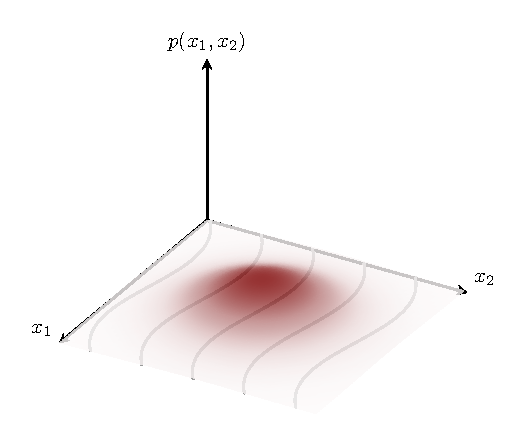
\includegraphics{figures/conditional_density_functions/discrete_partition/initial_density/initial_density.pdf}

}

\subcaption{\label{fig-discrete-conditional-initial}}

\end{minipage}%
%
\begin{minipage}{0.45\linewidth}

\centering{

\captionsetup{labelsep=none}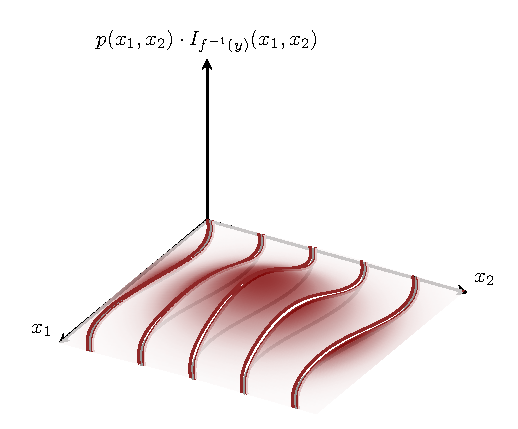
\includegraphics{figures/conditional_density_functions/discrete_partition/partitioned_densities/partitioned_densities.pdf}

}

\subcaption{\label{fig-discrete-conditional-partitioned}}

\end{minipage}%
%
\begin{minipage}{0.05\linewidth}
~\end{minipage}%
\newline
\begin{minipage}{0.28\linewidth}
~\end{minipage}%
%
\begin{minipage}{0.45\linewidth}

\centering{

\captionsetup{labelsep=none}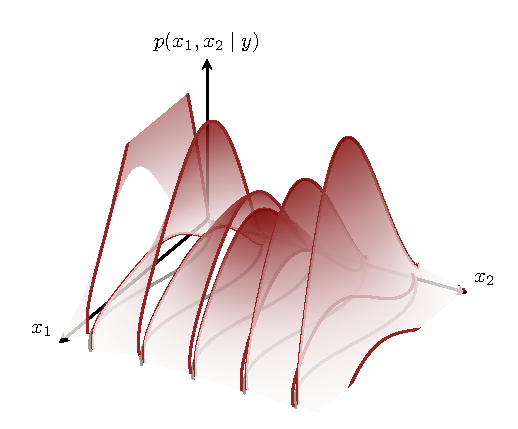
\includegraphics{figures/conditional_density_functions/discrete_partition/renormalized_densities/renormalized_densities.pdf}

}

\subcaption{\label{fig-discrete-conditional-renormalized}}

\end{minipage}%
%
\begin{minipage}{0.28\linewidth}
~\end{minipage}%

\caption{\label{fig-discrete-conditional}Conditional probability density
functions are straightforward to construct for countable partitions. (a)
A probability density function representing the initial probability
distribution is first (b) sliced into density functions restricted to
each level set. (c) Once properly normalized these density functions
become conditional probability density functions that represent each
conditional probability distribution.}

\end{figure}%

To double check our construction we can verity that this result is
consistent with each conditional probability density function
\(\pi^{f}_{y}\) completely concentrating on the corresponding level set,
\begin{align*}
\pi^{f}_{y}( f^{-1}(y) )
&=
\pi^{f}( f^{-1}(y) \mid y)
\\
&=
\int \mu( \mathrm{d} x) \, \frac{ \mathrm{d}  \pi^{f} }{ \mathrm{d}  \mu  }( x \mid y ) \,
I_{f^{-1}(y)}(x)
\\
&=
\int \mu( \mathrm{d} x) \,
\frac{ \frac{ \mathrm{d}  \pi }{ \mathrm{d}  \mu  }(x) \, I_{f^{-1}(y)}(x) }{ \pi ( f^{-1}(y) ) }
\,
I_{f^{-1}(y)}(x)
\\
&=
\frac{1}{ \pi ( f^{-1}(y) ) }
\int \mu( \mathrm{d} x) \, \frac{ \mathrm{d}  \pi }{ \mathrm{d}  \mu  }(x) \,
\left( I_{f^{-1}(y)}(x) \right)^{2}
\\
&=
\frac{1}{ \pi ( f^{-1}(y) ) }
\int \mu( \mathrm{d} x) \, \frac{ \mathrm{d}  \pi }{ \mathrm{d}  \mu  }(x) \,
I_{f^{-1}(y)}(x)
\\
&=
\frac{1}{ \pi ( f^{-1}(y) ) }
\pi( f^{-1}(y) )
\\
&=
1.
\end{align*} Equivalently for any measurable subset
\(\mathsf{x} \in \mathcal{X}\) that is disjoint with a particular level
set \(\mathsf{x} \cap f^{-1}(y) = \emptyset\) we have \begin{align*}
\pi^{f}_{y}( \mathsf{x} )
&=
\pi^{f}( \mathsf{x} \mid y)
\\
&=
\int \mu( \mathrm{d} x) \, \frac{ \mathrm{d}  \pi^{f} }{ \mathrm{d}  \mu  }( x \mid y ) \,
I_{\mathsf{x}}(x)
\\
&=
\int \mu( \mathrm{d} x) \,
\frac{ \frac{ \mathrm{d}  \pi }{ \mathrm{d}  \mu  }(x) \, I_{f^{-1}(y)}(x) }{ \pi ( f^{-1}(y) ) }
\,
I_{\mathsf{x}}(x)
\\
&=
\frac{1}{ \pi ( f^{-1}(y) ) }
\int \mu( \mathrm{d} x) \, \frac{ \mathrm{d}  \pi }{ \mathrm{d}  \mu  }(x) \,
I_{f^{-1}(y)}(x) \, I_{\mathsf{x}}(x)
\\
&=
\frac{1}{ \pi ( f^{-1}(y) ) }
\int \mu( \mathrm{d} x) \, \frac{ \mathrm{d}  \pi }{ \mathrm{d}  \mu  }(x) \,
I_{\mathsf{x} \cap f^{-1}(y) }(x)
\\
&=
\frac{1}{ \pi ( f^{-1}(y) ) }
\int \mu( \mathrm{d} x) \, \frac{ \mathrm{d}  \pi }{ \mathrm{d}  \mu  }(x) \,
I_{ \emptyset }(x)
\\
&=
\frac{1}{ \pi ( f^{-1}(y) ) } \cdot 0
\\
&=
0.
\end{align*}

\subsection{The Problem With Null
Partitions}\label{the-problem-with-null-partitions}

Unfortunately this construction doesn't carry over to functions with
more general output spaces that might contain an uncountably-infinite
number of points. In this case at least some, if not all, of the level
sets will be allocated vanishing probabilities, \[
\pi( f^{-1}(y) ) = 0.
\] At the same time \(\sigma\)-finite reference measures will allocate
vanishing measure to at least some, if not all, of the level sets, \[
\mu( f^{-1}(y) ) = 0.
\]

These behaviors immediately obstruct many steps in our construction of a
discrete conditional probability density function. For example when
\(\pi( f^{-1}(y) ) = 0\) the final definition of a discrete conditional
probability density function \[
\frac{ \mathrm{d}  \pi^{f} }{ \mathrm{d}  \mu  }( x \mid y )
\overset{ \mu }{ = }
\frac{ \frac{ \mathrm{d}  \pi }{ \mathrm{d}  \mu  }(x) \, I_{f^{-1}(y)}(x) }{ \pi ( f^{-1}(y) ) }
\] requires an ill-defined division by zero.

Problems, however, actually arise much earlier in the calculation. On
the right-hand side of the law of total expectation we cannot convert
the output expectation value over \(f_{*} \pi\) into a sum over
individual output elements if \(Y\) is uncountable. Similarly when \(Y\)
is uncountable we cannot apply the \emph{countable} linearity of
measure-informed integration to the constant function \[
1 = \sum_{y \in Y} I_{f^{-1}(y)}(x).
\]

The most fundamental of our problems is that when \(\mu(f^{-1}(y)) = 0\)
any probability distribution that is absolutely continuous with respect
to \(\mu\) must also allocate zero probability to \(f^{-1}(y)\). The
conditional probability distributions \(\pi^{f}_{y}\), however, allocate
not just a non-zero probability to the level set \(f^{-1}(y)\) but in
fact all of their probability! In other words the conditional
probability distributions are typically not absolutely continuous with
respect to \(\mu\), preventing us from converting conditional
expectation values into \(\mu\)-informed integrals weighted by a
conditional probability density function in the first place. Absolute
continuity is easy to disregard as unnecessarily abstract, but it has
important practical consequences like this!

Yet another way to see why we need a more general construction of
conditional probability theory is to assume that a probability density
function of a particular \(\pi^{f}_{y}\) with respect to \(\mu\) does
exist and show that a mathematical inconsistency arises. For example in
order to ensure that \[
\pi^{f}_{y}( f^{-1}(y) ) = \pi^{f}( f^{-1}(y) \mid y) = 1
\] we would need a conditional probability density function to satisfy
\begin{align*}
1
&=
\pi^{f}( f^{-1}(y) \mid y)
\\
&=
\int \pi^{f}( \mathrm{d} x \mid y) \, I_{f^{-1}(y)}(x)
\\
&=
\int \mu( \mathrm{d} x) \,
\frac{ \mathrm{d}  \pi^{f} }{ \mathrm{d}  \mu  }(x \mid y) \, I_{f^{-1}(y)}(x).
\end{align*}

If, however, \(\mu( f^{-1}(y) ) = 0\) then the indicator function will
be non-zero for only a \(\mu\)-null subset of inputs. Consequently in
terms of \(\mu\)-informed integrals it should be equivalent to the zero
function, \[
I_{f^{-1}(y)}(x) \overset{\mu}{=} 0.
\] This would require that \begin{align*}
\int \mu( \mathrm{d} x) \,
\frac{ \mathrm{d}  \pi^{f} }{ \mathrm{d}  \mu  }(x \mid y) \, I_{f^{-1}(y)}(x)
&=
\int \mu( \mathrm{d} x) \,
\frac{ \mathrm{d}  \pi^{f} }{ \mathrm{d}  \mu  }(x \mid y) \cdot 0
\\
&= 0.
\end{align*} Unfortunately \[
1 = \int \mu( \mathrm{d} x) \,
\frac{ \mathrm{d}  \pi^{f} }{ \mathrm{d}  \mu  }(x \mid y) \, I_{f^{-1}(y)}(x) = 0
\] is a pretty immediate mathematical contradiction.

Notice the similarity of this inconsistent behavior with the awkward
behavior we encountered when exploring the Dirac delta function in
\href{https://betanalpha.github.io/assets/chapters_html/density_functions.html}{Chapter
6, Section 5.1}. Intuitively when \(f^{-1}(y)\) is a \(\mu\)-null subset
the corresponding conditional probability distribution \(\pi^{f}_{y}\)
becomes singular, and probability density functions become ill-defined
without opening our hearts and minds to generalized functions like the
Dirac delta function.

One way to avoid this singular behavior is to embrace the interpretation
of each conditional probability distribution \(\pi^{f}_{y}\) being
defined over not all of the ambient space \(X\) but rather just the
corresponding level set \(f^{-1}(y)\). From this perspective we can
define conditional probability density functions with respect to
\(\sigma\)-finite reference measures defined on the level sets
themselves, \[
\int \pi^{f}( \mathrm{d} x \mid y ) \, g(x)
=
\int \nu_{y}( \mathrm{d} x ) \,
\frac{ \mathrm{d}  \pi^{f} }{ \mathrm{d}  \nu_{y}  } (x \mid y) \, g(x).
\] Incorporating these probability functions into the law of total
expectation, however, requires an explicit relationship between these
level set reference measures \(\nu_{y}\) to the ambient reference
measure \(\mu\). This, in turn, requires extending the disintegration of
probability measures to the disintegration of more general measures.

\subsection{Disintegrating Measures}\label{disintegrating-measures}

In \hyperref[sec:general-conditional]{Section 3.2} we introduced
disintegrations of probability distributions. This definition pretty
immediately generalizes to finite measures, which for mathematical
purposes are equivalent to probability distributions, but it becomes
problematic when working with non-finite measures. Even
\(\sigma\)-finite measures require some extra care to decompose across
null subsets.

The core mathematical issue is that a consistent disintegration of a
measure \(\mu\) with respect to a function \(f : X \rightarrow Y\)
requires not only that the initial measure \(\mu\) is \(\sigma\)-finite
but also that its pushforward \(f_{*} \mu\) is \(\sigma\)-finite.
Unfortunately this latter condition fails for many convenient reference
measures.

Consider, for example, a rigid two-dimensional real space
\(\mathbb{R}^{2}\) equipped with the two-dimensional Lebesgue measure
\(\lambda^{2}\) and a projection function \begin{alignat*}{6}
\varpi_{1} :\; &\mathbb{R}^{2}& &\rightarrow& \; &\mathbb{R}&
\\
&(x_{1}, x_{2})& &\mapsto& &x_{1}&.
\end{alignat*} The Lebesgue measure \(\lambda^{2}\) is
\(\sigma\)-finite, allocating finite measure to every measurable subset
that can be encapsulated in a finite rectangle. Formally if \[
\mathsf{x} \subset [0, 1] \times [0, 1]
\] then \begin{align*}
\lambda^{2}(\mathsf{x})
&<
\lambda^{2}( [0, 1] \times [0, 1] )
\\
&<
l([0, 1]) \cdot l([0, 1])
\\
&<
1 \cdot 1
\\
&<
1.
\end{align*}

Pushing \(\lambda^{2}\) forward along \(\varpi_{1}\), however, results
in a measure that allocates \emph{infinite} measure to finite intervals
(Figure~\ref{fig-lebesgue-pushforward}), \begin{align*}
(\varpi_{1})_{*} \lambda^{2} ( [0, 1] )
&=
\lambda^{2}( \varpi_{1}^{*} [0, 1])
\\
&= \lambda^{2}( [0, 1] \times (-\infty, \infty) )
\\
&= l([0, 1]) \cdot l( (-\infty, \infty) )
\\
&= 1 \cdot \infty
\\
&= \infty.
\end{align*} Consequently \((\varpi_{1})_{*} \lambda^{2}\) cannot be
\(\sigma\)-finite.

\begin{figure}

\centering{

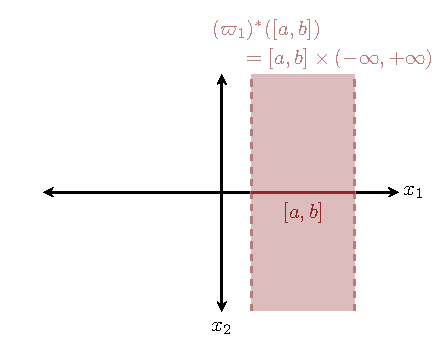
\includegraphics[width=0.5\textwidth,height=\textheight]{figures/lebesgue_pushforward/lebesgue_pushforward.pdf}

}

\caption{\label{fig-lebesgue-pushforward}On \(\mathbb{R}^{2}\) the
projection function \(\phi_{1} : (x_{1}, x_{2}) \mapsto x_{1}\) pulls
back finite intervals \([a, b]\) into infinite rectangles
\([a, b] \times (-\infty, +\infty)\). Consequently the two dimensional
Lebesgue measure \(\lambda^{2}\) projects infinite measure onto finite
intervals and the pushforward measure \((\phi_{1})_{*} \lambda^{2}\)
cannot be \(\sigma\)-finite. In particular \(\lambda^{2}\) does
\emph{not} pushforward to a Lebesgue measure!}

\end{figure}%

Fortunately disintigrations can be generalized to work with not only the
pushforward of the target measure but also \emph{any} convenient
\(\sigma\)-finite measure on the output space. Mathematically if we have

\begin{enumerate}
\def\labelenumi{\arabic{enumi}.}
\tightlist
\item
  an input measurable space \((X, \mathcal{X})\),
\item
  a \(\sigma\)-finite Radon measure
  \(\mu : \mathcal{X} \rightarrow [0, \infty]\),
\item
  an output Hausdorff measurable space \((Y, \mathcal{Y})\).
\item
  a surjective measurable function
  \(f: (X, \mathcal{X}) \rightarrow (Y, \mathcal{Y})\),
\item
  and finally a \(\sigma\)-finite measure
  \(\nu : \mathcal{Y} \rightarrow [0, \infty]\)
\end{enumerate}

then there exists at least one \textbf{conditional measure kernel}
\begin{alignat*}{6}
\mu^{f, \nu} :\; &\mathcal{X} \times Y& &\rightarrow& \; &[0, \infty]&
\\
&\mathsf{x}, y& &\mapsto& &\mu^{f}( \mathsf{x} \mid y )&
\end{alignat*} that defines a
\((\mathcal{Y}, \mathcal{B}_{\mathbb{R}})\)-measurable function when
partially evaluated on the first argument, \begin{alignat*}{6}
\mu^{f, \nu}_{\mathsf{x}} :\; &Y& &\rightarrow& \; &[0, \infty]&
\\
&y& &\mapsto& &\mu^{f, \nu}( \mathsf{x} \mid y )&
\end{alignat*} for all \(\mathsf{x} \in \mathcal{X}\), and a
\(\sigma\)-finite measure when partially evaluated on the second
argument, \begin{alignat*}{6}
\mu^{f}_{y, \nu} :\; &\mathcal{X}& &\rightarrow& \; &[0, \infty]&
\\
&\mathsf{x}& &\mapsto& &\mu^{f, \nu}( \mathsf{x} \mid y )&
\end{alignat*} for \(\nu\)-almost all \(y \in Y\). A more technical
discussion can be found in Chang and Pollard (1997).

The conditional measures derived from a conditional measure kernel
behave very similarly to conditional probability distributions. For
example they each concentrate on a particular level set, \[
\mu^{f, \nu}_{y}( f^{-1}(x) ) \overset{\nu}{=} 1
\] with \[
\mu^{f, \nu}_{y}( \mathsf{x} ) \overset{\nu}{=} 0
\] for any \(\mathsf{x} \in \mathcal{X}\) with
\(\mathsf{x} \cap f^{-1}(y) = \emptyset\). They also satsify a law of
total integration, \[
\int \mu( \mathrm{d} x ) \, g(x)
=
\int \nu (\mathrm{d} y)
\int \mu^{f, \nu}( \mathrm{d}x_{y} \mid y ) \, g(x),
\] for any well-behaved integrand \(g : X \rightarrow \mathbb{R}\).

In circumstances where \(f_{*} \mu\) happens to be \(\sigma\)-finite we
can always take \(\nu = f_{*} \mu\) so that the law of total integration
mirrors the law of total expectation. This is always possible if \(\mu\)
is a finite measure, and hence always possible when disintegrating
probability distributions, but it is not always viable when \(\mu\) is
only \(\sigma\)-finite. In particular we have to be vigilent when
attempting to disintegrate the Lebesgue and counting measures that we
often turn to for convenient reference measures as they often
pushforward to measures that are not \(\sigma\)-finite.

\subsection{Conditional Probability Density Functions For General
Implicit
Partitions}\label{conditional-probability-density-functions-for-general-implicit-partitions}

Armed with a technique for disintegrating \(\sigma\)-finite measures we
are now finally equipped with enough tools to construct conditional
probability density functions for any conditional probability
distribution and sufficiently well-behaved reference measure.

Recall that to construct a conditional probability distribution we need

\begin{enumerate}
\def\labelenumi{\arabic{enumi}.}
\tightlist
\item
  an input measurable space \((X, \mathcal{X})\),
\item
  a Radon probability distribution
  \(\pi : \mathcal{X} \rightarrow [0, 1]\),
\item
  an output Hausdorff measurable space \((Y, \mathcal{Y})\).
\item
  and a surjective measurable function
  \(f: (X, \mathcal{X}) \rightarrow (Y, \mathcal{Y})\).
\end{enumerate}

In order to construct conditional probability density functions we will
also need convenient \(\sigma\)-finite Radon reference measures for

\begin{enumerate}
\def\labelenumi{\arabic{enumi}.}
\setcounter{enumi}{4}
\tightlist
\item
  the input space, \(\mu : \mathcal{X} \rightarrow [0, \infty]\),
\item
  the output space, \(\nu : \mathcal{Y} \rightarrow [0, \infty]\),
\item
  and each level set,
  \(\eta_{y} : \mathcal{F}_{y} \rightarrow [0, \infty]\).
\end{enumerate}

As we have previously discussed we can safely take measurable functions,
Hausdorff \(\sigma\)-algebras, and Radon measures for granted in
practice. We will, however, have to be careful about the surjectivity of
\(f\) and the \(\sigma\)-finiteness of the reference measures.

If \(\pi \ll \mu\) then we can construct the probability density
function \[
\frac{ \mathrm{d}  \pi }{ \mathrm{d}  \mu  } : X \rightarrow \mathbb{R}^{+},
\] and if \(f_{*} \pi \ll \nu\) then we can construct the pushforward
probability density function \[
\frac{ \mathrm{d}  f_{*} \pi }{ \mathrm{d}  \nu  } : Y \rightarrow \mathbb{R}^{+}.
\] Upon disintegrating \(\mu\) we can also construct the conditional
probability density functions relative to the conditional measures, \[
\frac{ \mathrm{d}  \pi^{f} }{ \mathrm{d}  \mu^{f, \nu}  }
: X \times Y \rightarrow \mathbb{R}^{+}.
\] Finally if \(\mu^{f, \nu}_{y} \ll \eta_{y}\) then we can convert
these conditional probability density functions into conditional
probability density functions relative to our level set reference
measures, \[
\frac{ \mathrm{d}  \pi^{f} }{ \mathrm{d}  \eta_{y}  } (x \mid y)
\overset{ \eta_{y} }{=}
\frac{ \mathrm{d}  \pi^{f} }{ \mathrm{d}  \mu^{f, \nu}  } (x \mid y)
\cdot
\frac{ \mathrm{d}  \mu^{f, \nu} }{ \mathrm{d}  \eta_{y}  } (x \mid y).
\] In many applications the conditional measures \(\mu^{f, \nu}_{y}\)
will be convenient reference measures and we will not need to consider
an auxiliarycollection of reference measures \(\eta_{y}\). That said
here I will consider the more general scenario for completeness.

All that we're missing is a mathematical relationship that ties this
menagerie of probability density functions together. That information is
hidden within the law of total expectation, \begin{align*}
\int \pi( \mathrm{d} x ) \, g(x)
&=
\int f_{*} \pi (\mathrm{d} y)
\int \pi^{f}( \mathrm{d}x_y \mid y ) \, g(y, x_{y})
\\
L
&=
R.
\end{align*} All we need to do is convert both sides of this equation
into the same kind of measure-informed integral.

Let's start with the left-hand side, \begin{align*}
L
&=
\int \pi ( \mathrm{d} x ) \, g(x)
\\
&=
\int \mu ( \mathrm{d} x ) \, \frac{ \mathrm{d} \pi}{ \mathrm{d} \mu }(x) \, g(x).
\end{align*} If we disintegrate \(\mu\) with respect to \(f\) and
\(\nu\) this becomes \begin{align*}
L
&=
\int \mu ( \mathrm{d} x ) \, \frac{ \mathrm{d} \pi}{ \mathrm{d} \mu }(x) \, g(x)
\\
&=
\int \nu ( \mathrm{d} y ) \,
\int \mu^{f, \nu}( \mathrm{d} x_{y} \mid y) \,
\frac{ \mathrm{d} \pi}{ \mathrm{d} \mu }(y, x_{y}) \, g(y, x_{y}).
\end{align*} Incorporating the level set reference measures then gives
\begin{align*}
L
&=
\int \nu ( \mathrm{d} y ) \,
\int \mu^{f, \nu}( \mathrm{d} x_{y} \mid y) \,
\frac{ \mathrm{d} \pi}{ \mathrm{d} \mu }(y, x_{y}) \, g(y, x_{y})
\\
&=
\int \nu ( \mathrm{d} y ) \,
\int \eta_{y} ( \mathrm{d} x_{y}) \,
\frac{ \mathrm{d} \mu^{f, \nu}}{ \mathrm{d} \eta_{y} }(x_{y} \mid y) \,
\frac{ \mathrm{d} \pi}{ \mathrm{d} \mu }(y, x_{y}) \, g(y, x_{y})
\\
&=
\int \nu ( \mathrm{d} y ) \,
\int \eta_{y} ( \mathrm{d} x_{y}) \,
\left[ \frac{ \mathrm{d} \mu^{f, \nu}}{ \mathrm{d} \eta_{y} }(x_{y} \mid y) \,
\frac{ \mathrm{d} \pi}{ \mathrm{d} \mu }(y, x_{y}) \right] \, g(y, x_{y}).
\end{align*}

Over on the right-hand side we have \begin{align*}
R
&=
\int f_{*} \pi (\mathrm{d} y)
\int \pi^{f}( \mathrm{d}x_{y} \mid y ) \, g(y, x_{y})
\\
&=
\int \nu (\mathrm{d} y) \,
\frac{ \mathrm{d}  f_{*} \pi }{ \mathrm{d}  \nu  }(y) \,
\int \pi^{f}( \mathrm{d}x_{y} \mid y ) \, g(y, x_{y})
\\
&=
\int \nu (\mathrm{d} y) \,
\frac{ \mathrm{d}  f_{*} \pi }{ \mathrm{d}  \nu  }(y) \,
\int \eta_{y} ( \mathrm{d}x_{y} ) \,
\frac{ \mathrm{d} \pi^{f}}{ \mathrm{d} \eta_{y} }(x_{y} \mid y) \, g(y, x_{y}).
\end{align*} Because the domain of the inner measure-informed integral
is single level set the pushforward probability density function
\(\mathrm{d} f_{*} \pi / \mathrm{d} \nu\) is a constant that can be
pulled inside, \begin{align*}
R
&=
\int f_{*} \pi (\mathrm{d} y)
\int \pi^{f}( \mathrm{d}x_{y} \mid y ) \, g(y, x_{y})
\\
&=
\int \nu (\mathrm{d} y) \,
\frac{ \mathrm{d}  f_{*} \pi }{ \mathrm{d}  \nu  }(y) \,
\int \eta_{y} ( \mathrm{d}x_{y} ) \,
\frac{ \mathrm{d} \pi^{f}}{ \mathrm{d} \eta_{y} }(x_{y} \mid y) \, g(y, x_{y})
\\
&=
\int \nu (\mathrm{d} y) \,
\int \eta_{y} ( \mathrm{d}x ) \,
\frac{ \mathrm{d}  f_{*} \pi }{ \mathrm{d}  \nu  }(y) \,
\frac{ \mathrm{d} \pi^{f}}{ \mathrm{d} \eta_{y} }(x_{y} \mid y) \, g(y, x_{y})
\\
&=
\int \nu (\mathrm{d} y) \,
\int \eta_{y} ( \mathrm{d}x )
\left[ \frac{ \mathrm{d}  f_{*} \pi }{ \mathrm{d}  \nu  }(y) \,
       \frac{ \mathrm{d} \pi^{f}}{ \mathrm{d} \eta_{y} }(x_{y} \mid y) \right] \, g(y, x_{y}).
\end{align*}

We can now put these two pieces back together, \begin{align*}
&
\quad\; L = R
\\
&
\int \pi( \mathrm{d} x ) \, g(x)
\\
&\quad\quad=
\int f_{*} \pi (\mathrm{d} y)
\int \pi^{f}( \mathrm{d}x_{y} \mid y ) \, g(y, x_{y})
\\
&
\int \nu ( \mathrm{d} y ) \,
\int \eta_{y} ( \mathrm{d} x_{y} ) \,
\left[ \frac{ \mathrm{d} \mu^{f, \nu}}{ \mathrm{d} \eta_{y} }(x_{y} \mid y) \,
\frac{ \mathrm{d} \pi}{ \mathrm{d} \mu }(y, x_{y}) \right] \, g(y, x_{y})
\\
&\quad\quad=
\int \nu (\mathrm{d} y) \,
\int \eta_{y} ( \mathrm{d}x_{y} )
\left[ \frac{ \mathrm{d}  f_{*} \pi }{ \mathrm{d}  \nu  }(y)
       \, \frac{ \mathrm{d} \pi^{f}}{ \mathrm{d} \eta_{y} }(x_{y} \mid y) \right] \, g(y, x_{y}).
\end{align*} Because both sides of the equation are the same kind of
measure-informed integral we have equality if and only if the integrands
on both sides are equal up to null subsets. In particular we have
equality for all integrands \(g : X \rightarrow \mathbb{R}\) if and only
if \begin{align*}
\frac{ \mathrm{d} \mu^{f, \nu}}{ \mathrm{d} \eta_{y} }(x_{y} \mid y) \,
\frac{ \mathrm{d} \pi}{ \mathrm{d} \mu }(y, x_{y})
\overset{ \nu, \eta_{y} }{ = }
\frac{ \mathrm{d}  f_{*} \pi }{ \mathrm{d}  \nu  }(y) \, \frac{ \mathrm{d} \pi^{f}}{ \mathrm{d} \eta_{y} }(x_{y} \mid y).
\end{align*}

Isolating the ambient probability density function gives \begin{align*}
\frac{ \mathrm{d} \pi}{ \mathrm{d} \mu }(y, x_{y})
&\overset{ \eta_{y} }{ = }
\frac{ \mathrm{d}  f_{*} \pi }{ \mathrm{d} \nu }(y) \,
\frac{ \frac{ \mathrm{d}  \pi^{f} }{ \mathrm{d}  \eta_{y}  } (x_{y} \mid y) }
{ \frac{ \mathrm{d}  \mu^{f, \nu} }{ \mathrm{d}  \eta_{y}  } (x_{y} \mid y) }
\\
\frac{ \mathrm{d} \pi}{ \mathrm{d} \mu }(y, x_{y})
&\overset{ \mu }{ = }
\frac{ \mathrm{d}  f_{*} \pi }{ \mathrm{d} \nu }(y) \,
\frac{ \mathrm{d}  \pi^{f} }{ \mathrm{d}  \mu^{f, \nu}  } (x_{y} \mid y),
\end{align*} or, in terms of unconditional variables, \[
\frac{ \mathrm{d} \pi}{ \mathrm{d} \mu }(x)
\overset{ \mu }{ = }
\frac{ \mathrm{d}  f_{*} \pi }{ \mathrm{d} \nu }(f(x)) \,
\frac{ \mathrm{d}  \pi^{f} }{ \mathrm{d}  \mu^{f, \nu}  } (x \mid f(x)).
\] This relationship is known as the \textbf{product rule} for
probability density functions. The product rule allows to construct the
ambient probability density function, the conditional probability
density function, or the pushforward probability density function given
the other two. For example if we know the ambient probability density
function and the pushforward probability density function then the
conditional probability density function is given by \[
\frac{ \mathrm{d}  \pi^{f} }{ \mathrm{d}  \mu^{f, \nu}  } (x_{y} \mid y)
\overset{ \mu }{ = }
\frac{ \frac{ \mathrm{d} \pi}{ \mathrm{d} \mu }(y, x_{y}) }{ \frac{ \mathrm{d}  f_{*} \pi }{ \mathrm{d} \nu }(y) }.
\]

In words we can conditional a probability density function
\(\mathrm{d} \pi / \mathrm{d} \mu\) to a particular output point
\(y \in Y\) in two steps. First we restrict the inputs of
\(\mathrm{d} \pi / \mathrm{d} \mu\) to the points in the level set
\(f^{-1}(y)\) (Figure~\ref{fig-continuous-conditional-partitioned}\}).
Then we divide by the outputs of \(\mathrm{d} \pi / \mathrm{d} \mu\) by
the pushforward probability density function evaluated at \(y\),
\(\frac{ \mathrm{d}  f_{*} \pi }{ \mathrm{d} \nu }(y)\)
(Figure~\ref{fig-continuous-conditional-renormalized}).

\begin{figure}

\begin{minipage}{0.05\linewidth}
~\end{minipage}%
%
\begin{minipage}{0.45\linewidth}

\centering{

\captionsetup{labelsep=none}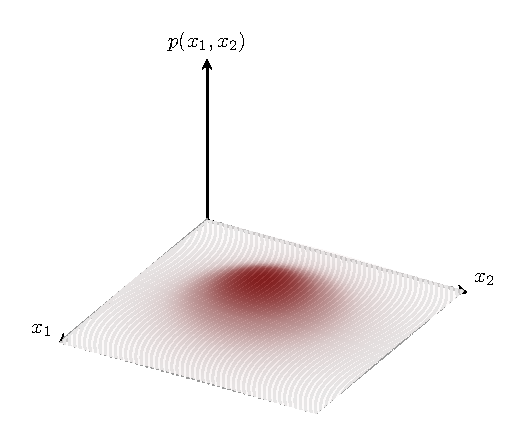
\includegraphics{figures/conditional_density_functions/continuous_partition/initial_density/initial_density.pdf}

}

\subcaption{\label{fig-continuous-conditional-initial}}

\end{minipage}%
%
\begin{minipage}{0.45\linewidth}

\centering{

\captionsetup{labelsep=none}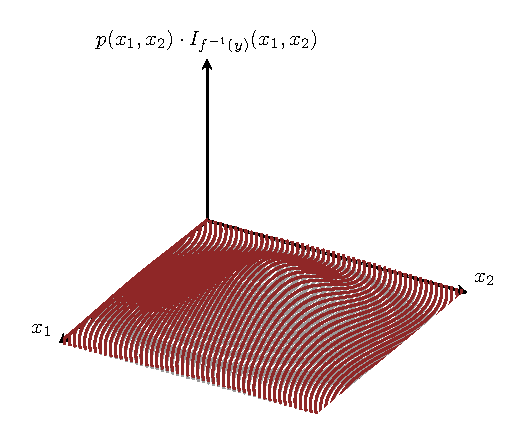
\includegraphics{figures/conditional_density_functions/continuous_partition/partitioned_densities/partitioned_densities.pdf}

}

\subcaption{\label{fig-continuous-conditional-partitioned}}

\end{minipage}%
%
\begin{minipage}{0.05\linewidth}
~\end{minipage}%
\newline
\begin{minipage}{0.28\linewidth}
~\end{minipage}%
%
\begin{minipage}{0.45\linewidth}

\centering{

\captionsetup{labelsep=none}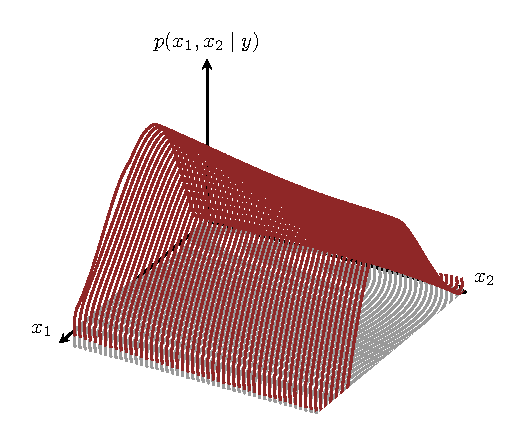
\includegraphics{figures/conditional_density_functions/continuous_partition/renormalized_densities/renormalized_densities.pdf}

}

\subcaption{\label{fig-continuous-conditional-renormalized}}

\end{minipage}%
%
\begin{minipage}{0.28\linewidth}
~\end{minipage}%

\caption{\label{fig-continuous-conditional}The product rule allows us to
generalize the construction of conditional probability density functions
that we first encountered in
\hyperref[sec:discrete-conditional-density]{Section 4.2}. (a) An initial
probability density function is first (b) sliced into a collection of
density functions by restricted inputs with non-zero outputs to
particular level set. (c) Dividing by the corresponding pushforward
probability density then normalizes these density functions into proper
conditional probability density functions.}

\end{figure}%

Notice, however, that this last step doesn't change the \emph{shape} of
the conditional probability density function, just its height. In
applications where we don't need to worry about the normalization we
ignore this last step, and any difficulty in evaluating the pushforward
probability density function, entirely.

To demonstrate this process consider a function
\(f : X \rightarrow \mathbb{N}\) that maps input points to output
integers and induces a countable partition. Because the output space is
discrete the counting measure is a natural output reference measure,
\(\nu = \chi\). Moreover if \(f_{*} \mu( \{ y \} ) > 0\) for all
\(y \in \mathbb{N}\) then each \(\mu^{f, \chi}_{y}\) becomes \(\mu\)
truncated to a particular level set, \[
\mu^{f, \chi}_{y} = \eta_{y} = I_{f^{-1}(y)} \cdot \mu.
\]

In this case the product rule gives \begin{align*}
\frac{ \mathrm{d}  \pi^{f} }{ \mathrm{d}  \mu^{f, \chi}  } (x_{y} \mid y)
&\overset{ \mu }{ = }
\frac{ \frac{ \mathrm{d} \pi}{ \mathrm{d} \mu }(y, x_{y}) }{ \frac{ \mathrm{d}  f_{*} \pi }{ \mathrm{d} \chi }(y) }
\\
&\overset{ \mu }{ = }
\frac{ \frac{ \mathrm{d} \pi}{ \mathrm{d} \mu }(y, x_{y}) }{ f_{*} \pi ( \{ y \} ) }
\\
&\overset{ \mu }{ = }
\frac{ \frac{ \mathrm{d} \pi}{ \mathrm{d} \mu }(y, x_{y}) }{ \pi ( f^{-1}(y) ) }.
\end{align*} For a given \(y \in Y\) we can extend these conditional
density functions to all inputs \(x \in X\) by returning zero outside of
the corresponding level set, \[
\frac{ \mathrm{d}  \pi^{f} }{ \mathrm{d}  \mu^{f, \chi}  } (x \mid y)
\overset{ \mu }{ = }
\left\{
\begin{array}{rr}
\frac{ \frac{ \mathrm{d} \pi}{ \mathrm{d} \mu }(x) }{ \pi ( f^{-1}(y) ) }, & x \in f^{-1}(y) \\
0, & x \notin f^{-1}(y)
\end{array}
\right. ,
\] or more compactly, \[
\frac{ \mathrm{d}  \pi^{f} }{ \mathrm{d}  \mu^{f, \chi}  } (x \mid y)
\overset{ \mu }{ = }
\frac{ \frac{ \mathrm{d} \pi}{ \mathrm{d} \mu }(x) \, I_{f^{-1}(y)}(x) }{ \pi ( f^{-1}(y) ) }.
\] This is encouragingly consistent with the result that we derived in
\hyperref[sec:discrete-conditional-density]{Section 4.2}.

\subsection{Explicit Formula For Pushforward Probability Density
Functions}\label{explicit-formula-for-pushforward-probability-density-functions}

The ability to disintegrate reference measures also gives us a way to
derive an explicit formula for pushforward probability density
functions.

Here we need to start with the definition of pullback expectation
values: for sufficiently-measurable functions \(f : X \rightarrow Y\)
and \(h : Y \rightarrow \mathbb{R}\) we have \begin{align*}
\mathbb{E}_{\pi} \! \left[  h \circ f  \right]
&=
\mathbb{E}_{f_{*} \pi} \! \left[  h  \right]
\\
\mathbb{I}_{\mu} \! \left[  \frac{ \mathrm{d}  \pi }{ \mathrm{d}  \mu  } \, h \circ f  \right]
&=
\mathbb{I}_{\nu} \! \left[  \frac{ \mathrm{d}  f_{*} \pi }{ \mathrm{d}  \nu  } \, h  \right]
\end{align*} or, equivalently, \begin{align*}
\int \pi( \mathrm{d} x ) \, h(f(x))
&=
\int f_{*} \pi( \mathrm{d} y )  \, h(y)
\\
\int \mu( \mathrm{d} x ) \, \frac{ \mathrm{d}  \pi }{ \mathrm{d}  \mu  }(x) \, h(f(x))
&=
\int \nu( \mathrm{d} y ) \, \frac{ \mathrm{d}  f_{*} \pi }{ \mathrm{d}  \nu  }(y) \, h(y).
\end{align*}

Disintegrating \(\mu\) with respect to \(f\) and \(\nu\) allows us to
write the left-hand side as \begin{align*}
\int \pi( \mathrm{d} x ) \, h(f(x))
&=
\int \mu( \mathrm{d} x ) \, \frac{ \mathrm{d} \pi}{ \mathrm{d} \mu }(x) \, h(f(x))
\\
&=
\int \nu( \mathrm{d} y ) \,
\int \mu^{f, \nu}( \mathrm{d} x_{y} \mid y ) \,
\frac{ \mathrm{d} \pi}{ \mathrm{d} \mu }(y, x_{y}) \, h(y).
\end{align*} Because the function
\(h \circ f : X \rightarrow \mathbb{R}\) yields the same output for any
\(x \in f^{-1}(y)\) it is a constant with respect to the inner integral
that can be factored out of the inner measure-informed integral,
\begin{align*}
\int \pi( \mathrm{d} x ) \, h(f(x))
&=
\int \nu( \mathrm{d} y ) \,
\int \mu^{f, \nu}( \mathrm{d} x_{y} \mid y ) \,
\frac{ \mathrm{d} \pi}{ \mathrm{d} \mu }(y, x_{y}) \, h(y)
\\
&=
\int \nu( \mathrm{d} y )
\left[ \int \mu^{f, \nu}( \mathrm{d} x_{y} \mid y )
       \, \frac{ \mathrm{d} \pi}{ \mathrm{d} \mu }(y, x_{y}) \right] \, h(y).
\end{align*}

Consequently \begin{align*}
\int \pi( \mathrm{d} x ) \, h(f(x))
&=
\int f_{*} \pi( \mathrm{d} y ) \, h(y)
\\
\int \nu( \mathrm{d} y )
\left[ \int \mu^{f, \nu}( \mathrm{d} x_{y} \mid y )
       \, \frac{ \mathrm{d} \pi}{ \mathrm{d} \mu }(y, x_{y}) \right] \, h(y)
&=
\int \nu( \mathrm{d} y ) \,
\left[ \frac{ \mathrm{d} f_{*}\pi}{ \mathrm{d} \nu }(y) \right] \, h(y).
\end{align*} Because both sides of this equation are \(\nu\)-informed
integrals we have equality if and only if the integrands are equal up to
\(\nu\)-null subsets. In particular we have equality for any integrand
\(h : Y \rightarrow \mathbb{R}\) if and only if \[
\frac{ \mathrm{d} f_{*}\pi}{ \mathrm{d} \nu }(y)
\overset{\nu}{=}
\int \mu^{f, \nu}( \mathrm{d} x_{y} \mid y ) \,
\frac{ \mathrm{d} \pi}{ \mathrm{d} \mu }(y, x_{y}).
\]

In theory this gives us an explicit formula for deriving pushforward
probability density functions. Implementing this result in practice,
however, will not be straightforward unless we happen to have an
explicit method for integrating the initial probability density function
over each level set of \(f\).

For example consider the two-dimensional space
\(X = \mathbb{R}^{+} \times \mathbb{R}^{+}\) equipped with a Lebesgue
probability density function \(p(x_{1}, x_{2})\) and the radial function
\begin{alignat*}{6}
f :\; &X& &\rightarrow& \; &\mathbb{R}^{+}&
\\
&(x_{1}, x_{2})& &\mapsto& &r = \sqrt{ x_{1}^{2} + x_{2}^{2} }&.
\end{alignat*}

The level sets of \(f\) define angular arcs of constant radius.
Conveniently these arcs are parameterized by a single variable if we
transform to polar coordinates
\(\mathbb{R}^{+} \times \left[ 0, \frac{\pi}{2} \right]\), with the map
\begin{align*}
r &= \sqrt{ x_{1}^{2} + x_{2}^{2} }
\\
\theta &= \arctan \left( \frac{ x_{2} }{ x_{1} } \right),
\end{align*} or equivalently \begin{align*}
x_{1} &= r \, \cos \theta
\\
x_{2} &= r \, \sin \theta.
\end{align*} In particular integrating over the variable \(\theta\)
implicitly for a particular \(r\) integrate over one of the angular
level sets.

To take advantage of this in practice we need to first transform the
initial probability density function \(p(x_{1}, x_{2})\) into the
probability density function \(p(r, \theta)\) using the Jacobian
correction that we encountered in
\href{https://betanalpha.github.io/assets/chapters_html/transforming_probability_spaces.html}{Chapter
7, Section 4.3.1}. After this transformation we integrate over
\(\theta\) to derive a pushforward probability density function over the
radial coordinate, \[
p(r)
=
\int_{0}^{\frac{\pi}{2}} \mathrm{d} \theta \, p(r, \theta).
\] Finally we can use the product rule to construct the conditional
probability density function over the angular level sets \[
p(\theta_{r} \mid r) = \frac{ p(r, \theta_{r}) }{ p(r) }.
\]

\begin{figure}

\begin{minipage}{0.05\linewidth}
~\end{minipage}%
%
\begin{minipage}{0.45\linewidth}

\centering{

\captionsetup{labelsep=none}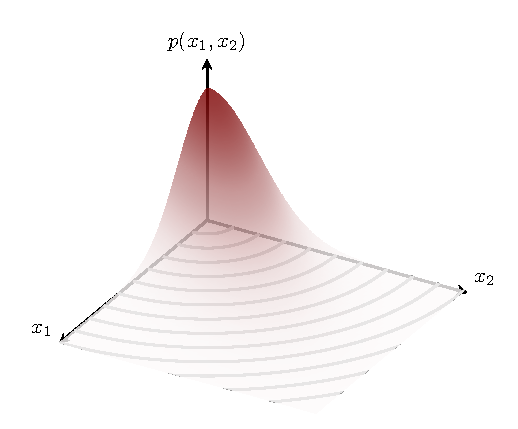
\includegraphics{figures/radial/initial/initial.pdf}

}

\subcaption{\label{fig-radial-initial}}

\end{minipage}%
%
\begin{minipage}{0.45\linewidth}

\centering{

\captionsetup{labelsep=none}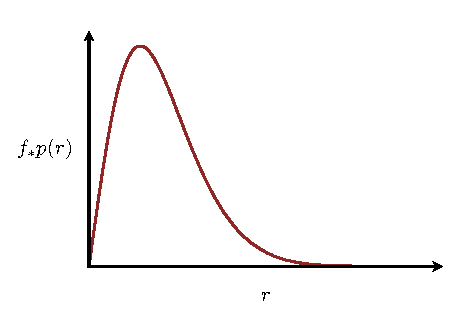
\includegraphics{figures/radial/pushforward/pushforward.pdf}

}

\subcaption{\label{fig-radial-pushforward}}

\end{minipage}%
%
\begin{minipage}{0.05\linewidth}
~\end{minipage}%
\newline
\begin{minipage}{0.28\linewidth}
~\end{minipage}%
%
\begin{minipage}{0.45\linewidth}

\centering{

\captionsetup{labelsep=none}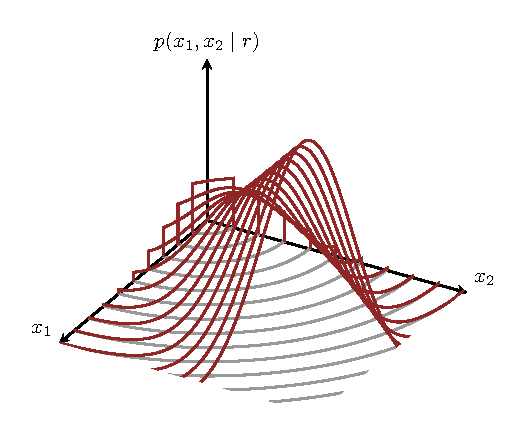
\includegraphics{figures/radial/conditional/conditional.pdf}

}

\subcaption{\label{fig-radial-conditional}}

\end{minipage}%
%
\begin{minipage}{0.28\linewidth}
~\end{minipage}%

\caption{\label{fig-radial}When we have the computational tools to
integrate over level sets we can evaluate pushforward probability
density functions, and hence conditional probability density functions.
Here we integrate (a) an initial density function (b) over circular arcs
to derive a pushforward probabilitiy density function over radii. (c)
Restricting the initial probabilty density function to angular level
sets and then dividing by pushforward probability densities then gives
conditional probability density functions over each angular level set.}

\end{figure}%

Implementing all of these calculations, however, is much easier said
than done. For those with a taste for tricky integrals I work through an
explicit example that requires some complicated mathematical functions
in the \href{@sec:appendix}{Appendix}.

\section{Conditional Building Blocks}\label{conditional-building-blocks}

To this point we have discussed conditional probability theory as a tool
for \emph{breaking} probability distributions down into simpler pieces.
Conditional probability theory, however, can also be used to
\emph{build} probability distributions up from simpler pieces.
Throughout I will continue to take the somewhat-obscure technical
requirements of Radon measures and Hausdorff \(\sigma\)-algebras for
granted.

Given a probability distribution \(\pi\) defined over the space \(X\)
and a measurable function \(f : X \rightarrow Y\) we can construct both
a pushforward probability distribution \(f_{*} \pi\) and a conditional
probability kernel \(\pi^{f}\). Through the laws of total probability
and total expectation these two byproducts allow us to reconstruct the
output of any probabilistic operation on \(\pi\).

This construction also works the other way around. Given a measurable
function \(f: X \rightarrow Y\) any probability distribution over the
output space \(\rho\) and conditional probability kernel
\begin{alignat*}{6}
\tau :\; &\mathcal{X} \times Y& &\rightarrow& \; &[0, 1]&
\\
&\mathsf{x}, y& &\mapsto& &\tau ( \mathsf{x} \mid y )&,
\end{alignat*} with \[
\tau ( f^{-1}(y) \mid y ) = 1
\] uniquely define a probability distribution \(\pi\) over \(X\) through
the law of total probability, \[
\pi( \mathsf{x} ) = \mathbb{E}_{\rho} [ t_{\mathsf{x}} ]
\] where \begin{alignat*}{6}
t_{\mathsf{x}} :\; &Y& &\rightarrow& \; &[0, 1]&
\\
&y& &\mapsto& &\tau ( \mathsf{x} \mid y )&.
\end{alignat*} In this case we say that \(\tau\) \textbf{lifts} \(\rho\)
into a probability distribution over \(X\).

Lifting allows us to construct probability distributions over \(X\)
sequentially, first specifying a probability distribution over a \(Y\)
and then filling in the missing information with conditional probability
distributions across the level sets of a function
\(f : X \rightarrow Y\). If \(Y\) is a much simpler space than \(X\),
for example a lower-dimensional space with fewer degrees of freedom to
consider, and the level sets of \(f\) are straightforward to interpret,
then this sequential procedure can be much easier to implement in
practice than trying to define a probability distribution directly on
\(X\).

Given a sequence of \(N + 1\) spaces, \[
\{ X_{0}, \ldots, X_{n}, \ldots, X_{N} \},
\] and functions relating them, \begin{align*}
f_{1} :& \, X_{0} \rightarrow X_{1}
\\
&\ldots
\\
f_{n} :& \, X_{n - 1} \rightarrow X_{n}
\\
&\ldots
\\
f_{N} :& \, X_{N - 1} \rightarrow X_{N},
\end{align*} we can even iterate this procedure, building up a
probability distribution over \(X_{0}\) from an initial probability
distribution over \(X_{N}\) and a sequence of conditional probability
kernels \[
\{ \tau_{N}, \ldots, \tau_{n}, \ldots, \tau_{1} \}.
\] This allows us to incrementally build up sophisticated probability
distributions over \(X_{0}\) from much simpler pieces. Iteratively
constructing probability distributions is particularly useful on product
spaces, which will be the topic of \textbf{Chapter 9}.

We can also define a lifted probability distribution through its
expectation values with the law of total expectation, \[
\int \pi( \mathrm{d} x ) \, g(x)
=
\int \rho (\mathrm{d} y)
\int \tau( \mathrm{d}x_{y} \mid y ) \, g(x).
\] The advantage of this latter approach is that it allows us to
implicitly define \(\pi\) through a sequence of probability density
functions.

Given an output reference measure \(\nu\) any sufficiently well-behaved
function \[
r : Y \rightarrow \mathbb{R}^{+}
\] with \(\mathbb{I}_{\nu}[ r ] = 1\) defines an output probability
distribution \(\rho = r \, \nu\) through the expectation values \[
\int \rho( \mathrm{d} y ) h(y)
=
\int \nu (\mathrm{d} y) \, r(y) \, h(y).
\] Similarly given an input reference measure \(\mu\) and its
disintegration \(\mu^{f, \nu}\) any sufficiently well-behaved binary
function \[
t : X \times Y \rightarrow \mathbb{R}^{+}
\] with \[
\mathbb{I}_{\mu^{f, \nu}_{y}}[ t ] \overset{\nu}{=} 1
\] defines a conditional probability kernel \(\tau = t \, \mu^{f, \nu}\)
through the conditional expectation values \[
\int \tau( \mathrm{d} x_{y} \mid y) \, g(y, x_{y})
=
\int \mu^{f, \nu}( \mathrm{d} x_{y} \mid y) \,
     \tau(x_{y} \mid y) \, g(y, x_{y}).
\] Finally the product of these two functions \[
p(x) = p(y, x_{y}) = t(x_{y} \mid y ) \, r( y )
\] will always satisfy \[
\mathbb{I}_{\mu} [ p ] = 1
\] and hence define an input probability distribution \(\pi = p \, \mu\)
through the expectation values \begin{align*}
\int \pi( \mathrm{d}x ) \, g(x)
&=
\int \rho (\mathrm{d}y)
\int \tau( \mathrm{d}x_{y} \mid y ) \, g(x)
\\
&=
\int \nu (\mathrm{d}x ) \, r(y) \,
\int \mu^{f, \nu}( \mathrm{d}x_{y} \mid y) \,
t(x_{y} \mid y) \, g(y, x_{y}).
\end{align*}

Iterating this construction over a sequence of spaces \[
\{ X_{0}, \ldots, X_{n}, \ldots, X_{N} \},
\] requires a sequence of functions, \[
f_{n} : X_{n - 1} \rightarrow X_{n},
\] an probability density function over the terminal space, \[
p_{N} : X_{N} \rightarrow \mathbb{R}^{+},
\] and a sequence of conditional probability density functions, \[
t_{n} : X_{n - 1} \times X_{n} \rightarrow \mathbb{R}^{+}.
\] Applying the product rule once gives a probability density function
over \(X_{N - 1}\), \[
p_{N - 1}(x_{N}, ( x_{N - 1})_{x_{N}} ) =
t_{N}( (x_{N - 1})_{x_{N}} \mid x_{N} ) \,
p_{N} (x_{N} ).
\] Repeating the product rule \(N - 1\) more times then gives a
probability density function over \(X_{0}\).

The conditional variable notation becomes a bit cumbersome here, so I'll
write this product as \begin{align*}
p_{0}(x_{0})
&=
t_{1}( x_{0} \mid x_{1} ) \cdots
t_{n}( x_{n - 1} \mid x_{n} ) \cdots
t_{N}( x_{N - 1} \mid x_{N} ) \, p_{N} (x_{N})
\\
&=
\left[ \prod_{n = 1}^{N} t_{n}( x_{n - 1} \mid x_{n} ) \right] \,
p_{N} (x_{N})
\end{align*} along with the recursive constraints \[
x_{n} = f_{n}( x_{n - 1} )
\] that completely fix the variables \(\{ x_{1}, \ldots, x_{N} \}\)
given a point \(x_{0}\).

In \textbf{Chapter 9} we'll introduce a more elegant notation that works
well in the special case of product spaces.

\section{Independence}\label{independence}

In general a probability distribution will induce different behavior on
different level sets of the conditioning function. The exceptional
cases, where the conditional behavior is the same for almost all level
sets, arises often enough in practical applications to be worthy of its
own terminology.

To start let's investigate what happens when conditioning not on a
single subset. In particular consider two measurable subsets
\(\mathsf{x}_{1} \in \mathcal{X}\) and
\(\mathsf{x}_{2} \in \mathcal{X}\) that have non-zero overlap with each
other, \[
\mathsf{x}_{1} \cap \mathsf{x}_{2} = \emptyset,
\] and are both allocated non-zero probability, \[
\pi(\mathsf{x}_{1}) > 0, \pi(\mathsf{x}_{2}) > 0.
\]

The conditional probability of the first subset given the second is, by
definition, \[
\pi( \mathsf{x}_{1} \mid \mathsf{x}_{2} )
=
\frac{ \pi( \mathsf{x}_{1} \cap \mathsf{x}_{2} ) }
{ \pi( \mathsf{x}_{2} ) }
\] In order for the conditioning to have no affect on how probability is
allocated to \(\mathsf{x}_{1}\) we need \begin{align*}
\pi( \mathsf{x}_{1} )
&=
\pi( \mathsf{x}_{1} \mid \mathsf{x}_{2} )
\\
\pi( \mathsf{x}_{1} )
&=
\frac{ \pi( \mathsf{x}_{1} \cap \mathsf{x}_{2} ) }
{ \pi( \mathsf{x}_{2} ) }
\end{align*} or \[
\pi( \mathsf{x}_{1} \cap \mathsf{x}_{2} )
=
\pi( \mathsf{x}_{1} ) \cdot \pi( \mathsf{x}_{2} )
\] When this condition holds we say that the two measurable subsets are
\textbf{independent} of each other with respect to the probability
distribution \(\pi\).

The independence of subsets, however, doesn't tell us anything about how
entire conditional probability distributions behave. For example we
might be tempted to consider the case where \emph{every} measurable
subset \(\mathsf{x} \in \mathcal{X}\) is independent of
\(\mathsf{x}_{2}\), \[
\pi ( \mathsf{x} \mid \mathsf{x}_{2} ) = \pi( \mathsf{x} ).
\] In this case the entire conditional probability distribution would
reduce to the initial probability distribution. Unfortunately a
condition this strong is hard to satisfy; in fact it holds only when
\(\mathsf{x}_{2} = X\) and we're not really constraining the initial
probability distribution in the first place.

A much more useful notion of independence is when almost all of the
conditional probability distributions in a conditional probability
kernel are equivalent, so the conditional behavior is independent of
whichever partition cell, level set, or output point we consider. To
rigorously define this notion of independence, however, we need the
level sets to be particularly well-behaved.

In general the level sets of a function don't need to share the same
topology. Most functions, however, exhibit level sets with uniform or
almost-uniform topologies. For example the level sets of the projection
function \begin{alignat*}{6}
\varpi :\; &\mathbb{R}^{2}& &\rightarrow& \; &\mathbb{R}&
\\
&(x_{1}, x_{2})& &\mapsto& &x_{1}&
\end{alignat*} are all real lines. Similarly the level sets of the
radial function \begin{alignat*}{6}
r :\; &\mathbb{R}^{2}& &\rightarrow& \; &\mathbb{R}^{+}&
\\
&(x_{1}, x_{2})& &\mapsto& &\sqrt{ x_{1}^{2} + x_{2}^{2} }&
\end{alignat*} are all circles except for the level set for
\(r(x_{1}, x_{2}) = 0\) which degenerates to a single point.

When the almost all of the level sets of a function share the same
topology then we can treat them as equivalent representations of some
common space \(L\), which we write as \[
f^{-1}(y) \equiv L.
\] In this case we can, at least in theory, construct conditional
probability kernels such that almost all of the conditional probability
distribution are equivalent to some common probability distribution over
\(L\), \[
\pi^{f}_{y} ( \mathsf{x}_{y} ) = \rho ( \mathsf{x}_{y} ).
\]

If the conditional probability kernel that we get by conditioning a
probabilty distribution \(\pi\) on a function \(f : X \rightarrow Y\)
behaves in this way then we say that \(\pi\) is \textbf{independent} of
\(f\). Again this does not mean that the conditional probability
distributions \(\pi^{f}_{y}\) behave exactly like \(\pi\) but rather
that \(f_{*} \pi\)-almost all of them behave exactly like each other. In
other words the behavior of \(\pi^{f}_{y}\) is independent of which
level set \(f^{-1}(y)\), and hence which output point \(y \in Y\), we
consider.

An immediate consequence of this definition is that if \(\pi\) is
independent of \(f\) then any conditional probability density functions
that we construct will not depend on \(y\) and the product rule becomes
\[
\frac{ \mathrm{d}  \pi }{ \mathrm{d}  \mu  } (y, x_{y})
\overset{\mu}{=}
\frac{ \mathrm{d}  \pi^{f} }{ \mathrm{d}  \mu^{f, \nu}  } (x_{y}) \,
\frac{ \mathrm{d}  f_{*} \pi }{ \mathrm{d}  \nu  } (y).
\] Here all of the output dependence is isolated to the pushforward
probability density function and all of the level set dependence is
isolated to a single conditional probability density function.

This result suggests a straightforward procedure for constructing
probability distributions that are independent of a given function
\(f : X \rightarrow Y\) whose level sets \(f^{-1}(y)\) are almost all
equivalent to some common space \(L\). Any function
\(r : Y \rightarrow \mathbb{R}^{+}\) with
\(\mathbb{I}_{\nu} \! \left[ r \right] = 1\) implicitly defines a
probability distribution over \(Y\) and any function
\(l : L \rightarrow \mathbb{R}^{+}\) with
\(\mathbb{I}_{\mu^{f, \nu}} \! \left[ l \right] = 1\) defines a
probability distribution over the common level set space. The product of
these two functions \(l(x_{y}) \cdot r(y)\) then defines a probability
distribution over \(X\) that is always independent of \(f\).

\section{Conclusion}\label{conclusion}

The intuition of conditional probability theory is relatively
straightforward: decomposing probability distributions into simpler
pieces. Implementing that intuition with consistent mathematics,
however, is much more complicated.

In this chapter we've worked through the key foundations of conditional
probability theory that will allow us to apply it to the discrete and
continuous spaces that we'll regularly encounter in practical
applications. That said the notation and terminology of this general
theory can be frustratingly dense.

Fortunately much of this frustration will be resolved in the next
chapter where we will apply conditional probability theory to product
spaces and their natural projection functions. In this particular
context much of the notation and terminology simplifies and conditional
probability theory becomes a much more productive tool.

\section*{Appendix: ``Explicit'' Calculations}\label{sec:appendix}
\addcontentsline{toc}{section}{Appendix: ``Explicit'' Calculations}

In this appendix I've sequestered some nasty integrals that arise when
we try to integrate over angular level sets to construct the pushforward
probability density function and the subsequent conditional probability
density functions shown in Figure~\ref{fig-radial}. This section is
completely optional and can be ignored without any consequence for
future chapters.

Consider the two-dimensional real space
\(X = \mathbb{R}^{+} \times \mathbb{R}^{+}\), the Lebesgue probability
density function \begin{align*}
p(x_{1}, x_{2})
&=
\frac{
\exp \left( - \frac{1}{2 \, s^{2}} \frac{1}{1 - \rho^{2}}
              ( x^{2} - 2 \, \rho \, x \, y + y^{2} ) \right)
}{
\int_{0}^{\infty} \int_{0}^{\infty}
\mathrm{d} x_{1} \, \mathrm{d} x_{2} \,
\exp \left( - \frac{1}{2 \, s^{2}} \frac{1}{1 - \rho^{2}}
             ( x^{2} - 2 \, \rho \, x \, y + y^{2} ) \right).
}
\\
&=
C \, \exp \left( - \frac{1}{2 \, s^{2}} \frac{1}{1 - \rho^{2}}
                   ( x^{2} - 2 \, \rho \, x \, y + y^{2} ) \right),
\end{align*} and the radial function \begin{alignat*}{6}
f :\; &X& &\rightarrow& \; &\mathbb{R}^{+}&
\\
&(x_{1}, x_{2})& &\mapsto& &r = \sqrt{ x_{1}^{2} + x_{2}^{2} }&.
\end{alignat*}

The level sets of \(f\) are given by angular arcs of constant radius.
Calculations over these level sets become much easier when we
reparameterize \(X\) into polar coordinates where the radial output
becomes one of the component parameters, and the position along the
corresponding arc becomes the other. This requires the transformation
\begin{align*}
r &= \sqrt{ x_{1}^{2} + x_{2}^{2} }
\\
\theta &= \arctan \left( \frac{ x_{2} }{ x_{1} } \right),
\end{align*} or equivalently \begin{align*}
x_{1} &= r \, \cos \theta
\\
x_{2} &= r \, \sin \theta.
\end{align*}

Applying the transformation rule for Lebesgue probability density
functions gives \begin{align*}
p(r, \theta)
&=
p( x_{1}(r, \theta), x_{2}(r, \theta) ) \,
\frac{1}{ | \mathrm{det} \, \mathbf{J}(r, \theta) | }
\\
&=
C \, \exp \left( - \frac{1}{2 \, s^{2}} \frac{1}{1 - \rho^{2}}
(   (r \, \cos \theta)^{2}
  - 2 \, \rho \, r \, \cos \theta \, r \, \sin \theta
  + (r \, \sin \theta)^{2} )
\right) \, r
\\
&=
C \, r \, \exp \left( - \frac{1}{2 \, s^{2}} \frac{1}{1 - \rho^{2}}
(   r^{2} \, \cos^{2} \theta
  - 2 \, \rho \, r^{2} \, \cos \theta \, \sin \theta
  + r^{2} \, \sin^{2} \theta )
\right)
\\
&=
C \, r \, \exp \left( - \frac{1}{2 \, s^{2}} \frac{r^{2}}{1 - \rho^{2}}
(   \sin^{2} \theta
  + \cos^{2} \theta
  - 2 \, \rho \, \sin \theta \, \cos \theta )
\right)
\\
&=
C \, r \, \exp \left( - \frac{1}{2 \, s^{2}} \frac{r^{2}}{1 - \rho^{2}}
( 1 - 2 \, \rho \, \sin \theta \, \cos \theta )
\right)
\\
&=
C \, r \, \exp \left( - \frac{1}{2 \, s^{2}} \frac{r^{2}}{1 - \rho^{2}}
( 1 - \rho \, \sin 2 \theta)
\right).
\end{align*}

In theory we can construct the pushforward probability density function
over the radial outputs of \(f\) by integrating out the angular
parameter, \begin{align*}
p(r)
&=
\int_{0}^{\frac{\pi}{2}} \mathrm{d} \theta \, p(r, \theta)
\\
&=
\int_{0}^{\frac{\pi}{2}} \mathrm{d} \theta \,
C \, r \, \exp \left( - \frac{1}{2 \, s^{2}} \frac{r^{2}}{1 - \rho^{2}}
( 1 - \rho \, \sin 2 \theta)
\right)
\\
&=
C \, r \,
\int_{0}^{\frac{\pi}{2}} \mathrm{d} \theta \,
\exp \left( - \frac{1}{2 \, s^{2}} \frac{r^{2}}{1 - \rho^{2}}
\right) \,
\exp \left( + \frac{1}{2 \, s^{2}} \frac{r^{2}}{1 - \rho^{2}} \,
              \rho \, \sin 2 \theta
\right)
\\
&=
C \, r \,
\exp \left( - \frac{1}{2 \, s^{2}} \frac{r^{2}}{1 - \rho^{2}} \right) \,
\int_{0}^{\frac{\pi}{2}} \mathrm{d} \theta \,
\exp \left( + \frac{r^{2}}{2 \, s^{2}} \frac{\rho}{1 - \rho^{2}} \,
              \sin 2 \theta
\right)
\\
&=
C \, r \,
\exp \left( - \frac{1}{2 \, s^{2}} \frac{r^{2}}{1 - \rho^{2}} \right) \,
\iota(r, \rho, \theta).
\end{align*}

Conveniently this integral can be reduced to special functions, albeit
not necessarily common ones, \begin{align*}
\iota(r, \rho, \theta)
&=
\int_{0}^{\frac{\pi}{2}} \mathrm{d} \theta \,
\exp \left( + \frac{r^{2}}{2 \, s^{2}} \frac{\rho}{1 - \rho^{2}} \,
              \sin 2 \theta
\right)
\\
&=
\frac{1}{2} \int_{0}^{\pi} \mathrm{d} \phi \,
\exp \left( + \frac{r^{2}}{2 \, s^{2}} \frac{\rho}{1 - \rho^{2}} \,
              \sin \phi \right)
\\
&=
\frac{\pi}{2} \left(
  I_{0} \left( \frac{r^{2}}{2 \, s^{2}} \frac{\rho}{1 - \rho^{2}} \right)
+ L_{0} \left( \frac{r^{2}}{2 \, s^{2}} \frac{\rho}{1 - \rho^{2}} \right)
\right)
\end{align*} where \(I_{0}(x)\) is the \textbf{zeroth-order modified
Bessel function of the first kind} and \(L_{0}(x)\) is the
\textbf{zeroth-order modified Struve function}.

Using this result the radial probability density function becomes
\begin{align*}
p(r)
&=
C \, r \,
\exp \left( - \frac{1}{2 \, s^{2}} \frac{r^{2}}{1 - \rho^{2}} \right) \,
\iota(r, \rho, \theta)
\\
&=
\frac{\pi}{2} \, C \, r \,
\exp \left( - \frac{1}{2 \, s^{2}} \frac{r^{2}}{1 - \rho^{2}} \right) \,
\left(
  I_{0} \left( \frac{r^{2}}{2 \, s^{2}} \frac{\rho}{1 - \rho^{2}} \right)
+ L_{0} \left( \frac{r^{2}}{2 \, s^{2}} \frac{\rho}{1 - \rho^{2}} \right)
\right).
\end{align*}

We can now use this pushforward probability density function to
construct the conditional probability density function over the radial
level sets, \[
p(x_{1}, x_{2} \mid r) = \frac{ p(x_{1}, x_{2}) }{ p(r) }.
\] That said the conditional probability density functions simplify
quite a bit if we work in polar coordinates where the angular coordinate
completely parameterizes the level sets, \begin{align*}
p(\theta \mid r)
&=
p(r, \theta \mid r)
\\
&=
\frac{ p(r, \theta) }{ p(r) }
\\
&=
\frac{
C \, r \, \exp \left( - \frac{1}{2 \, s^{2}} \frac{r^{2}}{1 - \rho^{2}}
( 1 - \rho \, \sin 2 \theta) \right)
}{
\frac{\pi}{2} \, C \, r \,
\exp \left( - \frac{1}{2 \, s^{2}} \frac{r^{2}}{1 - \rho^{2}} \right) \,
\left(
  I_{0} \left( \frac{r^{2}}{2 \, s^{2}} \frac{\rho}{1 - \rho^{2}} \right)
+ L_{0} \left( \frac{r^{2}}{2 \, s^{2}} \frac{\rho}{1 - \rho^{2}} \right)
\right)
}
\\
&=
\frac{
\exp \left( - \frac{1}{2 \, s^{2}} \frac{r^{2}}{1 - \rho^{2}}
( 1 - \rho \, \sin 2 \theta) \right)
}{
\frac{\pi}{2} \,
\exp \left( - \frac{1}{2 \, s^{2}} \frac{r^{2}}{1 - \rho^{2}} \right) \,
\left(
  I_{0} \left( \frac{r^{2}}{2 \, s^{2}} \frac{\rho}{1 - \rho^{2}} \right)
+ L_{0} \left( \frac{r^{2}}{2 \, s^{2}} \frac{\rho}{1 - \rho^{2}} \right)
\right)
}
\\
&=
\frac{2}{\pi} \,
\frac{
\exp \left( - \frac{1}{2 \, s^{2}} \frac{r^{2}}{1 - \rho^{2}}
              ( 1 - \rho \, \sin 2 \theta)
            + \frac{1}{2 \, s^{2}} \frac{r^{2}}{1 - \rho^{2}} \right)
}{
  I_{0} \left( \frac{r^{2}}{2 \, s^{2}} \frac{\rho}{1 - \rho^{2}} \right)
+ L_{0} \left( \frac{r^{2}}{2 \, s^{2}} \frac{\rho}{1 - \rho^{2}} \right)
}
\\
&=
\frac{2}{\pi} \,
\frac{
\exp \left( - \frac{1}{2 \, s^{2}} \frac{r^{2}}{1 - \rho^{2}}
(- \rho \, \sin 2 \theta) \right)
}{
  I_{0} \left( \frac{r^{2}}{2 \, s^{2}} \frac{\rho}{1 - \rho^{2}} \right)
+ L_{0} \left( \frac{r^{2}}{2 \, s^{2}} \frac{\rho}{1 - \rho^{2}} \right)
}
\\
&=
\frac{2}{\pi} \,
\frac{
\exp \left( + \frac{r^{2}}{2 \, s^{2}} \frac{\rho}{1 - \rho^{2}} \,
              \sin 2 \theta \right)
}{
  I_{0} \left( \frac{r^{2}}{2 \, s^{2}} \frac{\rho}{1 - \rho^{2}} \right)
+ L_{0} \left( \frac{r^{2}}{2 \, s^{2}} \frac{\rho}{1 - \rho^{2}} \right)
}.
\end{align*}

Note that this construction ensures that each individual conditional
probability density function is properly normalized, \begin{align*}
\int_{0}^{\frac{\pi}{2}} \mathrm{d} \theta \, p(\theta \mid r)
&=
\int_{0}^{\frac{\pi}{2}} \mathrm{d} \theta \,
\frac{2}{\pi} \,
\frac{
\exp \left( + \alpha \, \sin 2 \theta \right)
}{
  I_{0} \left( \alpha \right) + L_{0} \left( \alpha \right)
}
\\
&=
\frac{2}{\pi} \,
\frac{1}{
  I_{0} \left( \alpha \right) + L_{0} \left( \alpha \right)
}
\int_{0}^{\frac{\pi}{2}} \mathrm{d} \theta \,
\exp \left( + \alpha \, \sin 2 \theta \right)
\\
&=
\frac{1}{\pi} \,
\frac{1}{
  I_{0} \left( \alpha \right) + L_{0} \left( \alpha \right)
}
\int_{0}^{\pi} \mathrm{d} \phi \,
\exp \left( + \alpha \, \sin \phi \right)
\\
&=
\frac{1}{\pi} \,
\frac{1}{
  I_{0} \left( \alpha \right) + L_{0} \left( \alpha \right)
}
\pi \left(
  I_{0} \left( \alpha \right) + L_{0} \left( \alpha \right)
\right)
\\
&=
\frac{\pi}{\pi} \,
\frac{
  I_{0} \left( \alpha \right) + L_{0} \left( \alpha \right)
}{
  I_{0} \left( \alpha \right) + L_{0} \left( \alpha \right)
}
\\
&=
1,
\end{align*} where \[
\alpha = \frac{r^{2}}{2 \, s^{2}} \frac{\rho}{1 - \rho^{2}}.
\]

\section*{Acknowledgements}\label{acknowledgements}
\addcontentsline{toc}{section}{Acknowledgements}

A very special thanks to everyone supporting me on Patreon: Adam
Fleischhacker, Adriano Yoshino, Alessandro Varacca, Alexander Noll,
Alexander Petrov, Alexander Rosteck, Andrea Serafino, Andrew Mascioli,
Andrew Rouillard, Andrew Vigotsky, Ara Winter, Austin Rochford, Avraham
Adler, Ben Matthews, Ben Swallow, Benoit Essiambre, Bradley Kolb,
Brandon Liu, Brendan Galdo, Brynjolfur Gauti Jónsson, Cameron Smith,
Canaan Breiss, Cat Shark, Charles Naylor, Charles Shaw, Chase Dwelle,
Chris Jones, Christopher Mehrvarzi, Colin Carroll, Colin McAuliffe,
Damien Mannion, dan mackinlay, Dan W Joyce, Dan Waxman, Dan Weitzenfeld,
Daniel Edward Marthaler, Darshan Pandit, Darthmaluus, David Galley,
David Wurtz, Denis Vlašiček, Doug Rivers, Dr.~Jobo, Dr.~Omri Har
Shemesh, Dylan Maher, Ed Cashin, Edgar Merkle, Eric LaMotte, Ero
Carrera, Eugene O'Friel, Felipe González, Fergus Chadwick, Finn
Lindgren, Florian Wellmann, Geoff Rollins, Guido Biele, Håkan Johansson,
Hamed Bastan-Hagh, Haonan Zhu, Hector Munoz, Henri Wallen, hs, Hugo
Botha, Ian, Ian Costley, idontgetoutmuch, Ignacio Vera, Ilaria
Prosdocimi, Isaac Vock, J, J Michael Burgess, jacob pine, Jair Andrade,
James C, James Hodgson, James Wade, Janek Berger, Jason Martin, Jason
Pekos, Jason Wong, Jeff Burnett, Jeff Dotson, Jeff Helzner, Jeffrey
Erlich, Jesse Wolfhagen, Jessica Graves, Joe Wagner, John Flournoy,
Jonathan H. Morgan, Jonathon Vallejo, Joran Jongerling, JU, Justin Bois,
Kádár András, Karim Naguib, Karim Osman, Kejia Shi, Kristian Gårdhus
Wichmann, Lars Barquist, lizzie , LOU ODETTE, Luís F, Marcel Lüthi,
Marek Kwiatkowski, Mark Donoghoe, Markus P., Martin Modrák, Márton
Vaitkus, Matt Moores, Matthew, Matthew Kay, Matthieu LEROY, Mattia
Arsendi, Maurits van der Meer, Michael Colaresi, Michael DeWitt, Michael
Dillon, Michael Lerner, Mick Cooney, N Sanders, N.S. , Name, Nathaniel
Burbank, Nic Fishman, Nicholas Clark, Nicholas Cowie, Nick S, Octavio
Medina, Oliver Crook, Olivier Ma, Patrick Kelley, Patrick Boehnke, Pau
Pereira Batlle, Peter Johnson, Pieter van den Berg, ptr, Ramiro
Barrantes Reynolds, Raúl Peralta Lozada, Ravin Kumar, Rémi, Riccardo
Fusaroli, Richard Nerland, Robert Frost, Robert Goldman, Robert kohn,
Robin Taylor, Ryan Grossman, S Hong, Saleem Huda, Sean Wilson, Sergiy
Protsiv, Seth Axen, shira, Simon Duane, Simon Lilburn, sssz, Stan\_user,
Stephen Lienhard, Stew Watts, Stone Chen, Susan Holmes, Svilup, Tao Ye,
Tate Tunstall, Tatsuo Okubo, Teresa Ortiz, Theodore Dasher, Thomas
Kealy, Thomas Vladeck, Tiago Cabaço, Tim Radtke, Tobychev , Tom McEwen,
Tomáš Frýda, Tony Wuersch, Virginia Fisher, Vladimir Markov, Wil
Yegelwel, Will Farr, woejozney, yolhaj , yureq , Zach A, Zad Rafi, and
Zhengchen Cai.

\section*{References}\label{references}
\addcontentsline{toc}{section}{References}

\phantomsection\label{refs}
\begin{CSLReferences}{1}{0}
\bibitem[\citeproctext]{ref-ChangEtAl:1997}
Chang, Joseph T, and David Pollard. 1997. {``Conditioning as
Disintegration.''} \emph{Statistica Neerlandica} 51 (3): 287--317.

\bibitem[\citeproctext]{ref-LeaoEtAl:2004}
Leão Jr, D, M Fragoso, and P Ruffino. 2004. {``Regular Conditional
Probability, Disintegration of Probability and {R}adon Spaces.''}
\emph{Proyecciones (Antofagasta)} 23 (1): 15--29.

\end{CSLReferences}

\section*{License}\label{license}
\addcontentsline{toc}{section}{License}

A repository containing all of the files used to generate this chapter
is available on
\href{https://github.com/betanalpha/quarto_chapters/tree/main/8_conditional_probability_theory}{GitHub}.

The text and figures in this chapter are copyrighted by Michael
Betancourt and licensed under the
\href{https://creativecommons.org/licenses/by-nc/4.0/}{CC BY-NC 4.0
license}.



\end{document}
